\documentclass[11pt, a4paper]{article}

\usepackage[utf8]{inputenc}
\usepackage[T1]{fontenc}
\usepackage[margin=2.5cm]{geometry}
\usepackage{amsmath, amssymb}
\usepackage{booktabs}
\usepackage{longtable}
\usepackage{array}
\usepackage{calc}
\usepackage{xcolor}
\usepackage{listings}
\usepackage{hyperref}
\usepackage{parskip}
\usepackage{graphicx}
\usepackage{etoolbox}
\usepackage{float}

\graphicspath{{figs/}}

\newcommand{\doi}[1]{\href{https://doi.org/#1}{doi:#1}}

% ── Fortran listings style ───────────────────────────────────
\definecolor{codebg}{RGB}{248,248,248}
\definecolor{codecomment}{RGB}{100,100,100}
\definecolor{codekw}{RGB}{0,80,160}
\definecolor{codestr}{RGB}{160,0,0}

\lstdefinelanguage{Fortran90}{
  morekeywords={program,end,use,implicit,none,integer,double,precision,
                logical,character,allocatable,parameter,real,if,then,else,
                do,while,call,subroutine,function,return,exit,allocate,
                deallocate,write,read,open,close,len,size,max,min,abs,
                sum,sqrt,mod,int,dble,any,trim,type},
  sensitive=false,
  morecomment=[l]{!},
  morestring=[b]",
  morestring=[b]'
}

\lstdefinelanguage{Python}{
  morekeywords={def,return,for,if,else,elif,import,from,as,in,not,and,or,
                True,False,None,class,with,lambda,yield,pass,break,continue},
  sensitive=true,
  morecomment=[l]{\#},
  morestring=[b]",
  morestring=[b]'
}

\lstset{
  language=Fortran90,
  basicstyle=\ttfamily\small,
  backgroundcolor=\color{codebg},
  commentstyle=\color{codecomment}\itshape,
  keywordstyle=\color{codekw}\bfseries,
  stringstyle=\color{codestr},
  frame=single,
  framesep=4pt,
  rulecolor=\color{gray!40},
  breaklines=true,
  numbers=none,
  captionpos=b,
  xleftmargin=6pt,
  xrightmargin=6pt,
}

\begin{document}

\title{\textbf{Monte Carlo Simulation of a Simple Polymer Chain}\\
       \large Implementation Report}
\author{Project\_2026\_II}
\date{12 April 2026}
\maketitle
\tableofcontents
\newpage

\subsection{Project Overview}\label{project-overview}

In this assignment, our goal was to develop a Monte Carlo simulation
program to explore the conformational landscape of a 500-Carbon linear
polymer chain (polyethylene) with varying torsional angles. The
simulation generates the initial conformation (with \& without
Hydrogens), measures torsional energy rotations, end-to-end distance,
and intramolecular Lennard-Jones interactions, and finally analyzes \&
visualizes the results.

After creating a serial processing version of the program,
parallelization techniques involving both MPI and OpenMP were
incorporated. These were compared to the serial version to demonstrate
both their individual and combined High Performance Computing
capabilities \& benefits.

Many techniques taught in class were crucial in the development of this
program, including: - \textbf{Git/Github} as a code respository \&
teamwork coordination platform - \textbf{Makefile} to automate the
compilation and execution of the code - \textbf{Shell scripting} for
facilitating server deployment - \textbf{MPI \& openMP} to parallelize
the code - \textbf{Python} for post-processing and plotting
\subsection{Repository Structure}\label{repository-structure}

Github was used as our team's code repository management system, and
from the root of
\href{https://github.com/Eines-Informatiques-Avancades/Project_2026_II}{the
project}, the code is divided among 3 main folders: \texttt{src},
\texttt{results}, and \texttt{docs}.

\begin{itemize}
\tightlist
\item
  \texttt{src} contains:

  \begin{itemize}
  \tightlist
  \item
    Makefile \& shell scripts
  \item
    Various versions of the main program (serial \& parallel)
  \item
    A \texttt{confs} folder where initial configurations are stored and
    compile-time options can be controlled via a file called
    \texttt{input.dat}
  \item
    A \texttt{lib} folder where module source files, python analysis
    files, and plotting style dependencies reside (\emph{further detail
    below})
  \end{itemize}
\item
  \texttt{results} contains the output data from the simulations
\item
  \texttt{docs} contains documentation and reports, including
  \texttt{img} folder for embedded images
\end{itemize}

In addition to these folders, a customary \texttt{README} file is
included in the root directory detailing run instructions and code
dependencies/requirements. The bulk of the code is written in Fortran,
while the post-processing is done in Python.

\#\#\# Module Library Introduction The following modules support the
\emph{\texttt{main...f90}} files: - \texttt{energy.f90} \&
\texttt{energy\_all\_atoms.f90} - Permit \textbf{dual energy modes},
computing energetic contributions using either TraPPE-UA or OPLS-AA
(with effective backbone potentials) depending on the
\texttt{explicit\_h} toggle dynamically read from \texttt{input.dat}. -
\texttt{initial-conf.f90} - Generates initial configuration of the
polymer chain. - \texttt{io.f90} - File input/ouput module. -
\texttt{monte\_carlo.f90} - Provides the rotation algorithm and
subroutine MCS step used to update spatial configurations. -
\texttt{observables.f90} - Computes the structural observables:
End-to-end distance (\(R_{ee}\)), Radius of Gyration (\(R_g\)), and
torsion angles. - \texttt{parameters.f90} - Stores global parameters
abstracted from \emph{\texttt{main...f90}} code. Works in tandem with
\texttt{input.dat} settings. - \emph{\texttt{plot\_...py}} files -
Various scripts used for plotting observables and serial vs parallel
code comparisons. - \texttt{requirements.txt} - List of python module
dependencies. - \texttt{science.mplstyle} - stylized document used in
plotting to control visualization theme.

\subsection{Code Management via
Github}\label{code-management-via-github}

The project leader was responsible for reviewing all pull requests,
ensuring that the code followed the project guidelines, and merging the
code into the main branch. The team coordinated through a WhatsApp group
chat and would regularly check in on each other's progress. Everyone was
informed when code was merged so we could all pull the latest changes.

Most times, approving and merging was straightforward with no issues,
but there was an interesting challenge when multiple uploads from
different team members overlapped, causing conflicts. This forced us to
learn about stashing and rebasing to the newly updated master branch
before recommitting. The following process was ironed out to ensure a
smooth integration:

\begin{enumerate}
\def\labelenumi{\arabic{enumi}.}
\item
  Stash local (uncommitted) changes

\begin{Shaded}
\begin{Highlighting}[]
   \FunctionTok{git}\NormalTok{ stash}
\end{Highlighting}
\end{Shaded}
\item
  Pull latest changes from master branch

\begin{Shaded}
\begin{Highlighting}[]
   \FunctionTok{git}\NormalTok{ checkout master}
   \FunctionTok{git}\NormalTok{ pull main master}
\end{Highlighting}
\end{Shaded}
\item
  Rebase local changes onto master branch so it starts after the new
  merged code

\begin{Shaded}
\begin{Highlighting}[]
   \FunctionTok{git}\NormalTok{ checkout }\OperatorTok{\textless{}}\NormalTok{fork{-}feature}\OperatorTok{\textgreater{}}\NormalTok{/}\OperatorTok{\textless{}}\NormalTok{fork{-}branch}\OperatorTok{\textgreater{}}
   \FunctionTok{git}\NormalTok{ rebase master}
\end{Highlighting}
\end{Shaded}
\item
  Resolve any conflicts \& re-apply stashed changes

\begin{Shaded}
\begin{Highlighting}[]
   \FunctionTok{git}\NormalTok{ stash pop}
\end{Highlighting}
\end{Shaded}
\item
  Commit and push (using \texttt{-\/-force} parameter due to rebase)

\begin{Shaded}
\begin{Highlighting}[]
   \FunctionTok{git}\NormalTok{ push }\OperatorTok{\textless{}}\NormalTok{fork{-}remote}\OperatorTok{\textgreater{}} \OperatorTok{\textless{}}\NormalTok{fork{-}branch}\OperatorTok{\textgreater{}}\NormalTok{ {-}{-}force}
\end{Highlighting}
\end{Shaded}
\end{enumerate}

\subsection{Makefile}\label{makefile}

As the project evolved, so did the Makefile. Here are some of the
features we implemented:

Starting off, there are few main variables that control the compilation
process.... \begin{Shaded}
\begin{Highlighting}[]
\DataTypeTok{FC}       \CharTok{=}\StringTok{ gfortran}
\DataTypeTok{FFLAGS}   \CharTok{=}\StringTok{ {-}O2 {-}Wall {-}Wextra}
\DataTypeTok{OBJ\_DIR}  \CharTok{=}\StringTok{ ../bin}
\DataTypeTok{EXE}      \CharTok{=}\StringTok{ }\CharTok{$(}\DataTypeTok{OBJ\_DIR}\CharTok{)}\StringTok{/main\_serial.x}
\DataTypeTok{LIB\_OBJ}  \CharTok{=}\StringTok{ }\CharTok{$(}\DataTypeTok{OBJ\_DIR}\CharTok{)}\StringTok{/parameters.o }\CharTok{\textbackslash{}}
\StringTok{           }\CharTok{$(}\DataTypeTok{OBJ\_DIR}\CharTok{)}\StringTok{/io.o }\CharTok{\textbackslash{}}
\StringTok{           ...}
\DataTypeTok{MAIN\_OBJ} \CharTok{=}\StringTok{ }\CharTok{$(}\DataTypeTok{OBJ\_DIR}\CharTok{)}\StringTok{/main\_serial.o}

\DataTypeTok{NP}          \CharTok{?=}\StringTok{ 4}
\DataTypeTok{OMP\_THREADS} \CharTok{?=}\StringTok{ 2}
\end{Highlighting}
\end{Shaded}

\begin{itemize}
\tightlist
\item
  \texttt{FC}: Stands for ``Fortran Compiler''. We tell it to use
  gfortran.
\item
  \texttt{FFLAGS}: These are the compiler flags. \texttt{-O2} is the
  optimization schema, and \texttt{-Wall\ -Wextra} enables warnings.
\item
  \texttt{OBJ\_DIR} \& \texttt{EXE}: Defines the compiled binaries
  directory and the name of the final executable.
\item
  \texttt{LIB\_OBJ} \& \texttt{MAIN\_OBJ}: Defines the object files for
  the library and the main program.
\item
  \texttt{NP} \& \texttt{OMP\_THREADS}: Defines the number of processes
  (MPI) and threads (openMP) to use for the parallel version of the
  program. The default values are set to 4 and 2, respectively, but they
  can be overridden by setting them when compiling in the command line
  (e.g., \texttt{make\ run\_parallel\ NP=7\ OMP\_THREADS=3}).
\end{itemize}

In order to encompass both the serial and parallel versions of the
program, a check is performed on the \texttt{make} command entered on
the command-line for the word \texttt{parallel}. If found, the user's
system is searched to ensure the environment has the necessary MPI and
OpenMP libraries installed. If not, an error message is printed and the
program exits. If they are installed, the compiler variable \texttt{FC}
is overwritten and the MPI and OpenMP flags are added to the
\texttt{FFLAGS} variable.

\begin{Shaded}
\begin{Highlighting}[]
\ControlFlowTok{ifneq}\NormalTok{ (,}\CharTok{$(}\KeywordTok{findstring}\StringTok{ parallel}\KeywordTok{,}\CharTok{$(}\DataTypeTok{MAKECMDGOALS}\CharTok{))}\NormalTok{)}
  \CommentTok{\# MPI Compiler Wrapper Verification}
  \DataTypeTok{MPI\_BIN} \CharTok{:=}\StringTok{ }\CharTok{$(}\KeywordTok{shell}\StringTok{ command {-}v mpif90 2\textgreater{}/dev/null}\CharTok{)}
  \ControlFlowTok{ifeq}\NormalTok{ (}\CharTok{$(}\KeywordTok{strip}\StringTok{ }\CharTok{$(}\DataTypeTok{MPI\_BIN}\CharTok{))}\NormalTok{,)}
    \CharTok{$(}\KeywordTok{error}\StringTok{ "MPI Compiler is required but \textquotesingle{}mpif90\textquotesingle{} was not found! Please install it (e.g. \textquotesingle{}sudo apt install openmpi{-}bin\textquotesingle{})"}\CharTok{)}
  \ControlFlowTok{endif}
  \CommentTok{\# Overwrite Compiler for MPI parallelization flag linking}
  \DataTypeTok{FC} \CharTok{=}\StringTok{ mpif90}
\NormalTok{  ...}
\end{Highlighting}
\end{Shaded}

Instead of writing a rule for every single \texttt{.f90} file, a pattern
rule (with \texttt{\%}) is used.

\begin{Shaded}
\begin{Highlighting}[]
\DecValTok{$(OBJ\_DIR)/\%.o:}\DataTypeTok{ lib/\%.f90}
\ErrorTok{    }\CharTok{@}\FunctionTok{mkdir {-}p }\CharTok{$(}\DataTypeTok{OBJ\_DIR}\CharTok{)}
    \CharTok{$(}\DataTypeTok{FC}\CharTok{)} \CharTok{$(}\DataTypeTok{FFLAGS}\CharTok{)}\NormalTok{ {-}J}\CharTok{$(}\DataTypeTok{OBJ\_DIR}\CharTok{)}\NormalTok{ {-}I}\CharTok{$(}\DataTypeTok{OBJ\_DIR}\CharTok{)}\NormalTok{ {-}c }\CharTok{$\textless{}}\NormalTok{ {-}o }\CharTok{$@}
\end{Highlighting}
\end{Shaded}

\begin{itemize}
\tightlist
\item
  It says: ``To make any \texttt{.o} file in the object directory
  (\texttt{bin/}) from a matching \texttt{.f90} file in \texttt{lib/},
  run this command.''
\item
  \texttt{-c\ \$\textless{}}: Compiles the ``first dependency''
  (\texttt{\$\textless{}}, which is the \texttt{.f90} file) without
  linking (because that's done in the \texttt{\$(EXE)} target).
\item
  \texttt{-J\$(OBJ\_DIR)\ -I\$(OBJ\_DIR)}: Tells Fortran to put module
  \texttt{.mod} files in the \texttt{bin/} folder.
\end{itemize}

The following is an example of the \texttt{all} target (serial version
of the program) with its executable structure, which we then follow up
with the explicit dependencies to create the \texttt{.o} files for the
library modules and the main program

\begin{Shaded}
\begin{Highlighting}[]
\DecValTok{all:}\DataTypeTok{ }\CharTok{$(}\DataTypeTok{EXE}\CharTok{)}

\DecValTok{$(EXE):}\DataTypeTok{ }\CharTok{$(}\DataTypeTok{LIB\_OBJ}\CharTok{)}\DataTypeTok{ }\CharTok{$(}\DataTypeTok{MAIN\_OBJ}\CharTok{)}
\ErrorTok{    }\CharTok{@}\FunctionTok{mkdir {-}p }\CharTok{$(}\DataTypeTok{OBJ\_DIR}\CharTok{)}
    \CharTok{$(}\DataTypeTok{FC}\CharTok{)} \CharTok{$(}\DataTypeTok{FFLAGS}\CharTok{)}\NormalTok{ {-}o }\CharTok{$@} \CharTok{$(}\DataTypeTok{LIB\_OBJ}\CharTok{)} \CharTok{$(}\DataTypeTok{MAIN\_OBJ}\CharTok{)}

\DecValTok{$(OBJ\_DIR)/energy.o:}\DataTypeTok{ lib/energy.f90 }\CharTok{\textbackslash{}}
\DataTypeTok{                     }\CharTok{$(}\DataTypeTok{OBJ\_DIR}\CharTok{)}\DataTypeTok{/parameters.o}
\NormalTok{...}

\DecValTok{$(OBJ\_DIR)/main\_serial.o:}\DataTypeTok{ main\_serial.f90 }\CharTok{$(}\DataTypeTok{LIB\_OBJ}\CharTok{)}
\ErrorTok{    }\CharTok{@}\FunctionTok{mkdir {-}p }\CharTok{$(}\DataTypeTok{OBJ\_DIR}\CharTok{)}
    \CharTok{$(}\DataTypeTok{FC}\CharTok{)} \CharTok{$(}\DataTypeTok{FFLAGS}\CharTok{)}\NormalTok{ {-}J}\CharTok{$(}\DataTypeTok{OBJ\_DIR}\CharTok{)}\NormalTok{ {-}I}\CharTok{$(}\DataTypeTok{OBJ\_DIR}\CharTok{)}\NormalTok{ {-}c }\CharTok{$\textless{}}\NormalTok{ {-}o }\CharTok{$@}
\end{Highlighting}
\end{Shaded}... \begin{itemize}
\tightlist
\item
  \texttt{all}: This is the default target that needs \texttt{\$(EXE)}
  to exist.
\item
  \texttt{\$(EXE)}: To build the final executable, it needs all the .o
  files from the \texttt{../bin} folder, which it makes sure exists
  (\texttt{mkdir\ -p}), and then links them all together using
  \texttt{gfortran} or \texttt{mpif90} to output (\texttt{-o\ \$@}) the
  final program.

  \begin{itemize}
  \tightlist
  \item
    \textbf{Note}: The \texttt{@} symbol is used 2 different ways here:

    \begin{enumerate}
    \def\labelenumi{\arabic{enumi}.}
    \tightlist
    \item
      Before the \texttt{mkdir} command to suppress being printed to the
      terminal.
    \item
      As an automatic variable representing the target name
      (\texttt{\$(EXE)} in this case).
    \end{enumerate}
  \end{itemize}
\end{itemize}

Last, we declare the shortcut commands as \texttt{.PHONY} targets to
prevent conflicts with files that may have the same name as a target.

\begin{Shaded}
\begin{Highlighting}[]
\OtherTok{.PHONY:}\DataTypeTok{ all clean run figures pipeline}

\DecValTok{run:}\DataTypeTok{ all}
\ErrorTok{    }\CharTok{@}\FunctionTok{mkdir {-}p ../results}
    \CharTok{$(}\DataTypeTok{EXE}\CharTok{)}

\DecValTok{figures:}
\ErrorTok{    }\NormalTok{python lib/plot\_results.py}

\DecValTok{clean:}\DataTypeTok{ }
\ErrorTok{    }\NormalTok{rm {-}rf }\CharTok{$(}\DataTypeTok{OBJ\_DIR}\CharTok{)}\NormalTok{/*.o }\CharTok{$(}\DataTypeTok{OBJ\_DIR}\CharTok{)}\NormalTok{/*.mod }\CharTok{$(}\DataTypeTok{EXE}\CharTok{)}

\DecValTok{pipeline:}
\ErrorTok{    }\CharTok{$(}\DataTypeTok{MAKE}\CharTok{)}\NormalTok{ run}
    \CharTok{$(}\DataTypeTok{MAKE}\CharTok{)}\NormalTok{ figures}
\end{Highlighting}
\end{Shaded}

\begin{itemize}
\tightlist
\item
  This enables the following compile-time shortcuts:

  \begin{itemize}
  \tightlist
  \item
    \texttt{make\ run}: Automatically builds the code (\texttt{all}) and
    then executes it.
  \item
    \texttt{make\ figures}: Envokes python to generate the plots from
    the \texttt{../results} folder.
  \item
    \texttt{make\ clean}: Acts like a reset button, deleting all
    compiled files to start fresh.
  \item
    \texttt{make\ pipeline}: A neat wrapper we built to run the code and
    generate the python plots back-to-back.
  \end{itemize}
\end{itemize}

\subsection{Shell Scripting}\label{shell-scripting}
% Itxaso bit added + Arthur's explanation merged

Shell scripting was used to make our runs compatible with the CERQT2
cluster environment and to automate benchmarking. The scripts
initialize the runtime environment, load the required modules, and set
variables such as \texttt{OMP\_NUM\_THREADS}, \texttt{NSLOTS}, and
\texttt{MPLBACKEND=Agg} for stable non-interactive execution. They were
also used to automate parameter sweeps, build explicit trajectory
manifests for the observables analysis, and collect timing data into
summary files for MPI and OpenMP tests.

A qsub script \texttt{run\_collab.qsub} was also written during the
testing of the program to submit an individual portion of the simulation
to the HPC cluster. It involved loading the appropriate modules for that
queue, selecting a custom makefile (separate from the main program's
Makefile), indentifying the correct commandline arguments to pass at
compile time, and submit the mpirun command.
% Source ownership:
% - Itxaso 

% ============================================================
\section{Initial Configuration Generation}
\label{sec:initial_conf}
% ============================================================

\subsection{Internal-Coordinate Builder}

The \texttt{initial\_conf} module is responsible for generating the starting
conformation of the polyethylene chain. The builder uses a recursive
internal-coordinate approach: each successive carbon atom is placed by
specifying a fixed C--C bond length ($d = 1.54\,\text{\AA}$), a fixed C--C--C
bond angle ($\theta = 114^\circ$), and a selectable dihedral angle $\phi$.
A hard-sphere overlap check with threshold $r_{\min} = 2.0\,\text{\AA}$ is
performed after each placement to avoid unphysical self-intersections during
chain construction.

\begin{lstlisting}[caption={Core internal-coordinate placement loop in \texttt{initial\_conf.f90}.}]
! Place carbon i based on the last two accepted positions
do i = 4, n_carbons
  ! Bond vector from i-2 to i-1 (normalised)
  b1 = coords(i-1,:) - coords(i-2,:)
  b1 = b1 / vnorm(b1)

  ! Normal to the C(i-2)-C(i-1)-C(i) plane
  b0 = coords(i-2,:) - coords(i-3,:)
  n_vec = cross(b0, b1)
  if (vnorm(n_vec) > 1.0d-8) n_vec = n_vec / vnorm(n_vec)

  ! Proposed new position using dihedral phi
  d_vec = bond_length * (                          &
      -cos_theta * b1                              &
      + sin_theta * (cos_phi * n_vec               &
                   + sin_phi * cross(b1, n_vec)))

  candidate = coords(i-1,:) + d_vec

  ! Overlap check against all previously placed atoms
  overlap = .false.
  do j = 1, i-1
    if (vnorm(candidate - coords(j,:)) < r_min) then
      overlap = .true.
      exit
    end if
  end do
  if (.not. overlap) coords(i,:) = candidate
end do
\end{lstlisting}

When explicit hydrogens are requested (\texttt{explicit\_h = .true.}), two
hydrogen atoms are appended for each internal CH$_2$ group and one for each
terminal CH$_3$ group, giving $N_{\text{atoms}} = 3N_C + 2$ total atoms for
a chain of $N_C$ carbons. The hydrogen placement is based on a local tetrahedral
frame: instead of placing the H atoms coplanar with the C--C--C backbone (chemically inconsistent), they are positioned out of the
backbone plane at the correct tetrahedral angle of $\approx 109.5^\circ$.

\begin{lstlisting}[caption={Out-of-plane hydrogen placement for internal CH$_2$ groups.}]
! For each internal carbon i (not first or last):
! Build local orthonormal frame {b_fwd, perp, out_of_plane}
b_fwd = coords(i+1,:) - coords(i-1,:)
b_fwd = b_fwd / vnorm(b_fwd)

! Perpendicular to backbone, in the C(i-1)-C(i)-C(i+1) plane
b_back = coords(i-1,:) - coords(i,:)
b_back = b_back / vnorm(b_back)
perp   = b_back - sum(b_back*b_fwd)*b_fwd
if (vnorm(perp) > 1.0d-8) perp = perp / vnorm(perp)

! Out-of-plane direction (cross product)
out_of_plane = cross(b_fwd, perp)
out_of_plane = out_of_plane / vnorm(out_of_plane)

! Place H1 and H2 symmetrically out of plane (tetrahedral geometry)
! cos(109.5 deg) ~ -1/3  =>  sin(109.5 deg) ~ sqrt(8/9)
h1 = coords(i,:) + r_CH * ( (-1.0d0/3.0d0)*(-perp)  &
     + sqrt(8.0d0/9.0d0) * 0.5d0 * ( out_of_plane + b_fwd) )
h2 = coords(i,:) + r_CH * ( (-1.0d0/3.0d0)*(-perp)  &
     + sqrt(8.0d0/9.0d0) * 0.5d0 * (-out_of_plane + b_fwd) )
\end{lstlisting}

\subsection{Configuration Modes}

Five distinct initial configuration modes have been implemented, each designed
to probe a different region of the polymer's conformational space:

\begin{table}[h!]
\centering
\caption{Summary of implemented initial configuration types.}
\label{tab:conf_types}
\begin{tabular}{clp{9cm}}
\toprule
\texttt{conf\_type} & Name & Description \\
\midrule
1 & All-trans (planar) & All dihedrals set to $\phi = 0^\circ$; fully extended
                         zigzag chain. Maximum end-to-end distance. \\
2 & Random & Each dihedral drawn uniformly from $[-\pi,\,\pi]$; maximally
             disordered starting state. \\
3 & RIS-like discrete & Dihedrals assigned with probabilities reflecting the
                        Rotational Isomeric State model (trans, gauche$^+$,
                        gauche$^-$). \\
4 & Spring / helix & Progressive dihedral increment per bond, producing a
                     helical backbone (proposed by ai-murphy). \\
5 & Perturbed trans & Small random perturbation applied to the all-trans
                      geometry; slight out-of-plane deviation while remaining
                      close to the global minimum. \\
\bottomrule
\end{tabular}
\end{table}

\begin{figure}[h!]
  \centering
  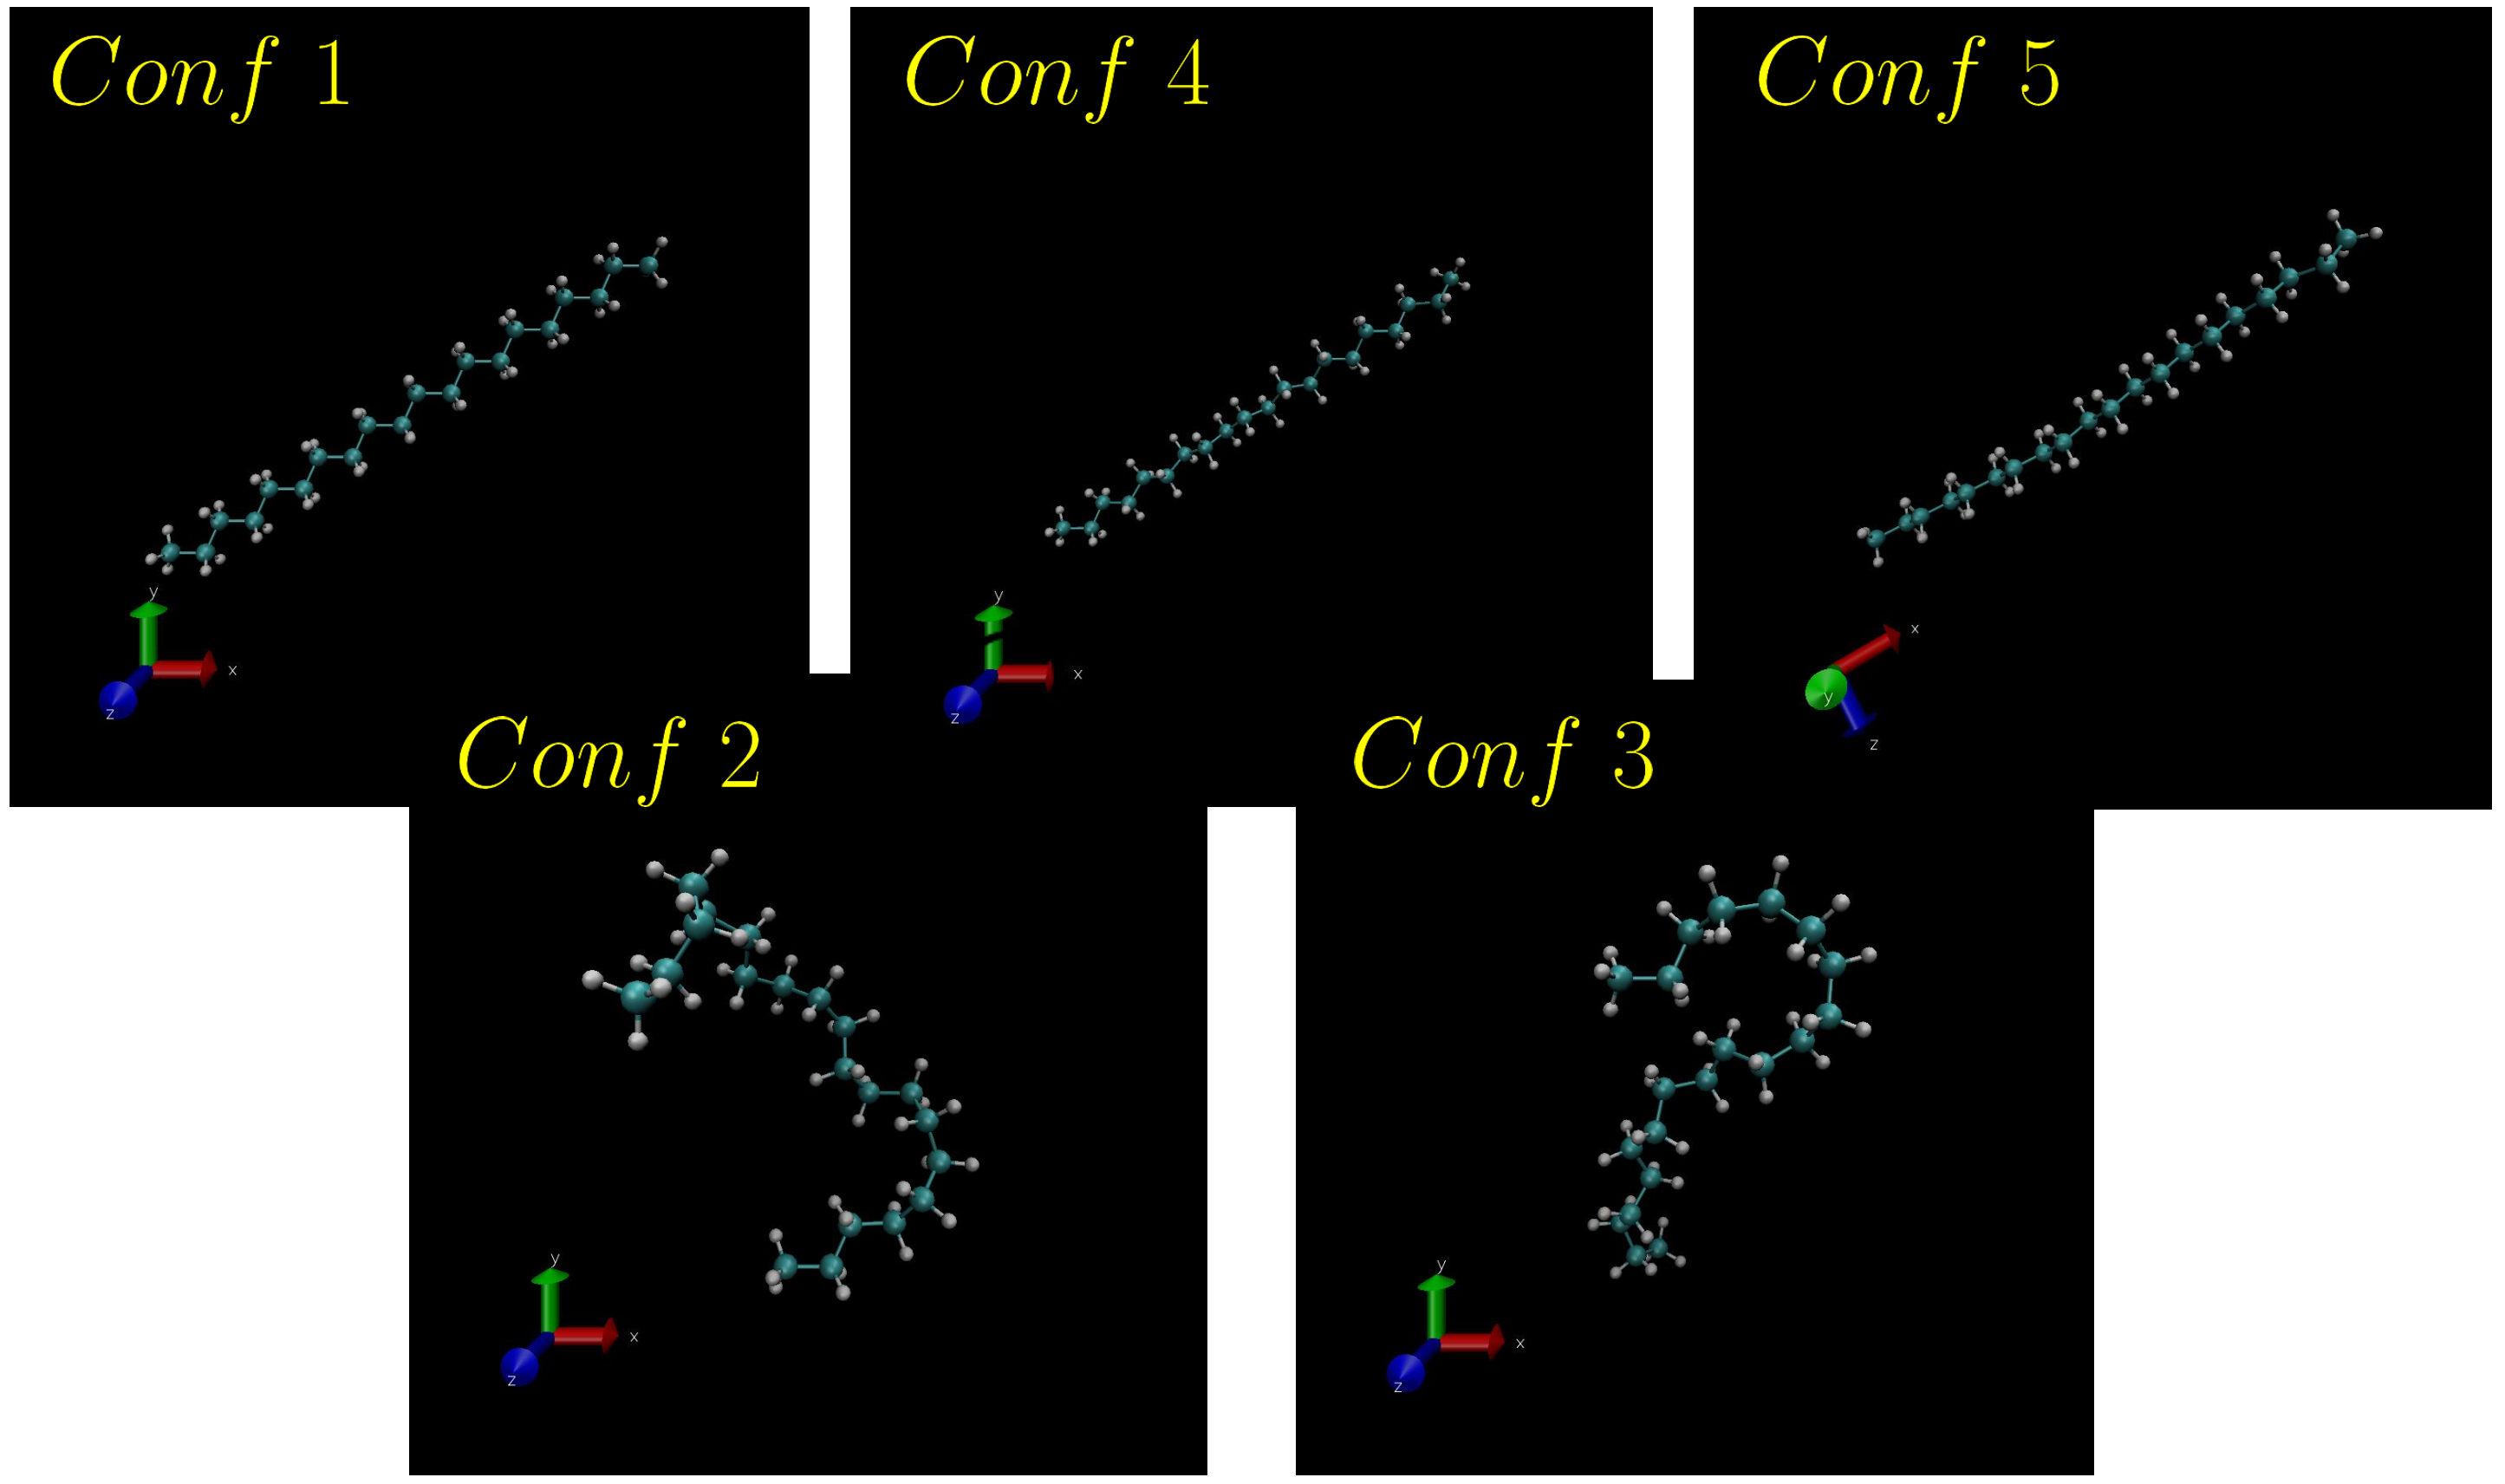
\includegraphics[width=\textwidth]{figs/INITIAL-CONFIGS.png}
  \caption{VMD snapshots of the five implemented initial configuration modes
  for the polyethylene chain. From left to right: (1) all-trans planar,
  (2) random, (3) RIS-like discrete, (4) spring/helix, and
  (5) perturbed trans.}
  \label{fig:initial_configs}
\end{figure}

Configurations 1 and 5 span the near-trans region of phase space, whereas
configurations 2 and 3 provide disordered starting points. Configuration 4 was
added to test helical initial geometries. Figure~\ref{fig:initial_configs}
provides a direct visual comparison of these starting states, illustrating the
broad structural diversity used to initialize the simulations.

This variety is relevant when the simulation is tested at different
temperatures: some initial states may lie closer to the equilibrated ensemble
than others, reducing the effective burn-in time.

% ============================================================
% Source ownership:
% - Itxaso

% ============================================================
\section{Input/Output Module}
\label{sec:io}
% ============================================================

\subsection{Parameter Parsing from \texttt{input.dat}}

All simulation parameters are read from a plain-text file \texttt{input.dat}
through the \texttt{io} module. The parser applies default values for any
missing keyword, strips inline comments (lines beginning with \texttt{\#}),
and performs basic range validation. The following parameters are controlled
from the input file:

\begin{table}[ht]
\centering
\caption{Simulation parameters read from \texttt{input.dat}.}
\label{tab:input_params}
\begin{tabular}{lll}
\toprule
Parameter & Default & Description \\
\midrule
\texttt{n\_carbons}   & 10       & Number of backbone carbon atoms \\
\texttt{n\_steps}     & 1{,}000{,}000 & Number of MC production steps \\
\texttt{temperature}  & 300.0    & Simulation temperature (K) \\
\texttt{conf\_type}   & 1        & Initial configuration mode (see Table~\ref{tab:conf_types}) \\
\texttt{explicit\_h}  & .false.  & Enable all-atom (explicit hydrogen) mode \\
\texttt{rng\_seed}    & 42       & Random number generator seed \\
\texttt{print\_interval} & 1{,}000 & Steps between output writes \\
\texttt{max\_delta}   & 0.5      & Maximum dihedral rotation per MC step (rad) \\
\midrule
\end{tabular}
\end{table}

Output is written in XYZ format: trajectories to
\texttt{traj\_\textit{label}.xyz}, energies to
\texttt{energy\_\textit{label}.dat}, and observables to
\texttt{observables\_\textit{label}.dat}, where the label encodes the key
simulation parameters (\texttt{n\_carbons}, \texttt{conf\_type},
\texttt{n\_steps}, \texttt{temperature}) for unambiguous identification.

% ============================================================
% Source ownership:
% - Oliwier: energy models, OPLS-AA, topology, delta_energy
% - Manel: Geweke runtime equilibration and MC workflow
% - Arthur: integration / prose cleanup

% - Keep modular because Oliwier will still update references

\section{Energy Evaluation and Monte Carlo Engine}
\label{sec:energy_mc}

\subsection{Energy Calculations}

The energy evaluation modules, \texttt{energy.f90} and \texttt{energy\_all\_atoms.f90}, were designed and implemented to compute the total potential energy of the chain and the $\Delta E$ increments required by the Metropolis acceptance/rejection step.

\subsubsection{United-Atom (UA) Model \& TraPPE-UA}

\textbf{Trigonometric bypass in dihedral calculations.}

The standard approach to evaluating a dihedral angle requires an
\texttt{acos} or \texttt{atan2} call, both of which are transcendental
functions with significant CPU cost relative to basic arithmetic.
Instead, \texttt{compute\_cos\_dihedral} computes $\cos\phi$ directly
from the dot product of the normal vectors of the two planes defined by
the carbon backbone:

\begin{equation}
  \cos\phi = \frac{\mathbf{n}_1 \cdot \mathbf{n}_2}{|\mathbf{n}_1|\,|\mathbf{n}_2|},
  \qquad
  \mathbf{n}_1 = \mathbf{b}_1 \times \mathbf{b}_2,\quad
  \mathbf{n}_2 = \mathbf{b}_2 \times \mathbf{b}_3
\end{equation}

where $\mathbf{b}_i$ are successive bond vectors. A guard clause handles
collinear atoms (degenerate normals) by setting $\cos\phi = 1$ as a
fallback. The function is declared \texttt{pure}, signalling to the compiler
that it has no side effects, which allows it to be called safely
from within parallel regions and \texttt{forall} constructs.

\textbf{Polynomial expansion for TraPPE-UA.}

The TraPPE-UA torsional potential~[3] is:

\begin{equation}
  U(\phi) = c_1(1+\cos\phi) + c_2(1-\cos 2\phi) + c_3(1+\cos 3\phi)
\end{equation}

Substituting $y = \cos\phi$ and applying the identities
$\cos 2\phi = 2y^2-1$ and $\cos 3\phi = 4y^3-3y$ gives a polynomial
in $y$:

\begin{equation}
  U(y) = c_1(1+y) + c_2(2-2y^2) + c_3(1-3y+4y^3)
\end{equation}

Since $y = \cos\phi$ is already available from the cross-product step,
the torsional energy is evaluated with only multiplications and
additions -- no further transcendental calls are needed in the MC loop.

\subsubsection{Explicit Hydrogens and the OPLS-AA Force Field}

The all-atom model requires handling a substantially more complex
topology. The OPLS-AA force field~[4] was adopted, with atom-specific
Lennard-Jones parameters for carbon and hydrogen
($\sigma_\mathrm{CC}=3.50\,\text{\AA}$,
$\varepsilon_\mathrm{CC}=0.066\,\text{kcal/mol}$;
$\sigma_\mathrm{HH}=2.50\,\text{\AA}$,
$\varepsilon_\mathrm{HH}=0.030\,\text{kcal/mol}$; cross-terms from
geometric mixing rules).

\textbf{Effective backbone torsional potential.}

In OPLS-AA, rotating a single C--C bond changes nine distinct dihedral
angles: one C--C--C--C, four C--C--C--H, and four H--C--C--H. Computing
all nine at every MC step is expensive for a code designed to run
millions of steps. An \emph{effective backbone potential} was therefore
constructed by summing the OPLS-AA Fourier coefficients for all nine
dihedral types analytically, producing a single set of effective
coefficients that reproduce the combined torsional energy from the
C--C--C--C backbone coordinates alone:

\begin{equation}
  c_1^\mathrm{eff} = 0.870,\quad
  c_2^\mathrm{eff} = -0.0785,\quad
  c_3^\mathrm{eff} = 1.5075 \quad \text{(kcal/mol)}
\end{equation}

The OPLS-AA Lennard-Jones parameters are taken from the framework of
Sæther et al.~[4]; the effective coefficient derivation is an original
contribution of this work. The same polynomial form used for the UA
model is then applied with these coefficients, so the all-atom
torsional evaluation has the same arithmetic cost as the united-atom one.

The corresponding \texttt{torsion\_single} function in
\texttt{energy\_all\_atoms.f90} is:

\begin{lstlisting}
pure function torsion_single(cos_phi) result(e)
  double precision, intent(in) :: cos_phi
  double precision :: e, y, y2, y3

  y  = cos_phi
  y2 = y * y
  y3 = y2 * y

  e = opls_c1 * (1.0d0 + y)            &
    + opls_c2 * (2.0d0 - 2.0d0 * y2)   &
    + opls_c3 * (1.0d0 - 3.0d0 * y + 4.0d0 * y3)
end function torsion_single
\end{lstlisting}

\textbf{Topology mapping and exclusion matrix.}

Non-bonded Lennard-Jones interactions must be suppressed for atom pairs
separated by fewer than four bonds (1-2, 1-3, and 1-4), since those
interactions are already captured by the bonded energy terms. The
initialisation routine \texttt{init\_energy\_topology} assigns each
hydrogen to its parent carbon by geometric distance (C--H threshold
$1.2\,\text{\AA}$), records the backbone position index for every atom,
and builds a global Boolean matrix \texttt{is\_excluded}. Each pair is
then looked up in $O(1)$ per call, avoiding any bond traversal during
the MC loop.

The exclusion criterion uses a uniform backbone-position threshold: pair
$(i,j)$ is excluded when
$|\text{backbone\_pos}(i) - \text{backbone\_pos}(j)| < 4$.
For C--C pairs this is exact. For C--H and H--H pairs the actual bond
count exceeds the backbone-position difference by one and two
respectively, so the threshold over-excludes some 1-5 and 1-6
interactions. The torsional potential partially compensates, since its
parameterisation implicitly encodes the conformational barriers arising
from steric repulsion. The single-chain, vacuum context of the
simulation further limits the practical impact relative to a condensed
phase. Correcting the exclusion criterion to a bond-count-aware rule is
left for future work.

\textbf{Dynamic atom lists for $\Delta E$.}

At each pivot move only atoms downstream of the chosen bond change
position. Recomputing the full $O(N^2)$ LJ sum is therefore unnecessary.
Instead, the atoms are partitioned into \texttt{fixed\_list} and
\texttt{moved\_list} by comparing old and new coordinate arrays:

\begin{lstlisting}
n_fixed = 0
n_moved = 0
do i = 1, n_atoms
  if (sum((coords_new(i,:) - coords_old(i,:))**2) > 1.0d-12) then
    n_moved = n_moved + 1
    moved_list(n_moved) = i
  else
    n_fixed = n_fixed + 1
    fixed_list(n_fixed) = i
  end if
end do
\end{lstlisting}

Only cross-interactions between fixed and moved atoms are re-evaluated,
reducing the $\Delta E$ cost to $O(N_\mathrm{fixed} \times
N_\mathrm{moved})$. A secondary \texttt{pair\_type\_matrix} routes each
valid pair to the pre-computed C--C, C--H, or H--H LJ parameters in a
single array lookup.

\subsection{Pivot Move and Monte Carlo Step}
 
The conformational sampling mechanism used throughout the project is the
pivot move. Rather than perturbing the whole chain diffusely, the
algorithm selects one internal C--C bond and rotates the entire tail of
the polymer as a rigid body around that bond axis. This generates large
collective rearrangements and allows the chain to explore configuration
space much more efficiently than local coordinate displacements.

The rigid-body rotation is implemented with Rodrigues' rotation formula.
If \(\mathbf{v}\) is the position of an atom relative to the pivot
point, \(\mathbf{k}\) is the unit vector along the selected bond, and
\(\theta\) is the random rotation angle, the rotated vector is
\[
\mathbf{v}_{\mathrm{rot}}
=
\mathbf{v}\cos\theta
+
(\mathbf{k}\times\mathbf{v})\sin\theta
+
\mathbf{k}(\mathbf{k}\cdot\mathbf{v})(1-\cos\theta).
\]
This construction preserves bond lengths and bond angles while applying
a clean rigid-body rotation to the selected downstream segment.

\subsubsection{Handling $sp^3$ Hybridisation in All-Atom Mode}

In all-atom mode, the same geometric transformation must be applied not
only to the carbon backbone but also to the hydrogens attached to every
rotating carbon. Because these hydrogens represent an approximately
tetrahedral $\mathrm{sp}^3$ environment, any inconsistency between the
carbon motion and the attached hydrogen motion would immediately distort
the local geometry and generate unphysical configurations. The AA
rotation routine therefore identifies the hydrogens attached to each
moving carbon and applies the exact same pivot point, axis, and angle to
them, using a C--H bond threshold of $1.2\,\text{\AA}$:
 
\begin{lstlisting}
if (explicit_h) then
  ! Hydrogens are stored after the carbon backbone in the coords array
  do i = n_carbons + 1, n_atoms
    do j = k + 1, n_carbons
      ! Identify if hydrogen i is bonded to the moving carbon j
      v = coords(i, :) - coords(j, :)
      if (vnorm(v) < 1.2d0) then
        ! Apply Rodrigues' rotation relative to the pivot point
        v = coords(i, :) - pivot
        dot_uv = sum(axis * v)
        v_rot = v * cos_p + cross(axis, v) * sin_p &
              + axis * dot_uv * (1.0d0 - cos_p)
        coords_new(i, :) = pivot + v_rot
        exit  ! Hydrogen found, move to the next atom
      end if
    end do
  end do
end if
\end{lstlisting}

\subsubsection{The MC Step and Metropolis Criterion}

Each call to \texttt{mc\_step} performs one trial move. First, a random
internal bond index $k$ is drawn uniformly from $[1,\, N_C - 2]$, and a
random rotation angle $\phi$ is sampled uniformly from
$[-\Delta\phi_{\max},\, \Delta\phi_{\max}]$; the parameter
\texttt{max\_delta} is tuned to achieve a reasonable acceptance rate.
Second, a trial configuration is generated by rotating the corresponding
tail segment while leaving the current coordinates unchanged. Third, the
change in energy is computed using the model-appropriate $\Delta E$
routine: \texttt{delta\_energy\_aa} for all-atom mode and
\texttt{delta\_energy\_ua} for united-atom mode, dispatched via the
\texttt{explicit\_h} flag. Fourth, the trial move is accepted or
rejected using the Metropolis criterion.

The Metropolis rule is standard. If the move lowers the total energy, it
is accepted unconditionally. Otherwise, it is accepted with probability
\[
P_{\mathrm{acc}} = \exp(-\beta \Delta E),
\qquad
\beta = \frac{1}{k_B T}.
\]
If accepted, the trial coordinates replace the current coordinates and
the total, Lennard-Jones, and torsional energies are updated in place.
If rejected, the trial geometry is discarded and the original state is
retained. Repeating this procedure generates a Markov chain whose
stationary distribution is the desired Boltzmann distribution.
 
\begin{lstlisting}
! d. Metropolis acceptance criterion
call random_number(random_value)
if (dE < 0.0d0 .or. random_value < exp(-beta * dE)) then
  coords  = coords_new
  E_total = E_total + dE
  E_lj    = E_lj    + dE_lj
  E_tors  = E_tors  + dE_tors
  accepted = .true.
end if
\end{lstlisting}
 
\subsection{Geweke Convergence Detection}

Detecting equilibration in a Markov chain is non-trivial because
successive configurations are strongly autocorrelated. Earlier versions
of the workflow relied on a fixed burn-in length and a posterior
post-processing check based on a Fast-Fourier Transform (FFT) script to
estimate the integrated autocorrelation time $\tau_\mathrm{int}$, but
this was often too rigid and could either discard too much data or fail
to detect persistent transients, sometimes reporting that the production
portion was 0\% of the 10M steps. To make equilibration detection
adaptive, the serial Monte Carlo engine was extended with an
in-simulation Geweke diagnostic~[1].

The Geweke test compares the mean of an early window of the trajectory
with the mean of a late window of the same trajectory. In our
implementation, the monitored quantity is the total energy. If the chain
has equilibrated, both windows should be consistent with the same
stationary distribution. The resulting $z$-score is
\[
z = \frac{\bar{x}_A - \bar{x}_B}
        {\sqrt{\mathrm{SE}_A^2 + \mathrm{SE}_B^2}},
\]
where $\bar{x}_A$ and $\bar{x}_B$ are the mean energies in the early
and late windows, and $\mathrm{SE}_A$ and $\mathrm{SE}_B$ are their
standard errors.

A crucial point is that the standard errors cannot be estimated from the
raw sample variance as if the measurements were independent. Monte Carlo
trajectories are correlated, so such a treatment would underestimate the
uncertainty and produce false positives. To account for this, the code
uses batch means. The window is partitioned into contiguous blocks, the
mean of each block is computed, and the variance of those block means is
used as an estimator of the uncertainty in the presence of
autocorrelation:

\begin{equation}
  SE_A^2 = \frac{1}{b_A(b_A-1)}\sum_{i=1}^{b_A}\left(\bar{x}_i - \bar{x}_A\right)^2
\end{equation}

where $\bar{x}_i$ is the mean of block $i$ and $\bar{x}_A$ is the mean
of the full window. $SE_B^2$ is computed analogously over window B.

The implementation uses an accumulated buffer of $N=300$ energy samples.
The early window contains the first $f_A=10\%$ of the buffer ($n_A=30$
samples, $b_A=\lfloor\sqrt{30}\rfloor=5$ blocks) and the late window
contains the last $f_B=50\%$ ($n_B=150$ samples,
$b_B=\lfloor\sqrt{150}\rfloor=12$ blocks). Because block means of
sufficiently large blocks behave approximately as independent, this
estimator correctly absorbs the autocorrelation structure of the chain.

Under the null hypothesis of stationarity, $z$ follows a standard
normal distribution. Equilibrium is declared when
$|z| < z_\mathrm{crit} = 1.96$ (95\% confidence level) on
$n_\mathrm{consec} = 3$ consecutive evaluations, preventing false
positives caused by temporary plateaus. The test is re-evaluated every
\texttt{eval\_freq} synchronisation points once the buffer is full,
so the simulation can stop the equilibration phase as soon as a
statistically stable regime has been reached. The production phase then
natively restarts step counting from 1.


% Source ownership:
% - Itxaso: Serial Driver and Scientific Output
% - Itxaso: Python Post-Processing and Analysis
% - Oliwier: cleaned serial-results narrative and figure placement

\section{Serial Driver, Results and Post-Processing}
\label{sec:serial_post}

\subsection{Two-Phase Simulation Structure}

The updated serial workflow is built around a two-phase execution model:
an adaptive equilibration stage followed by a fixed-length production
stage. This is implemented in \texttt{main\_serial\_equil.f90}, where the
program first reads \texttt{input.dat}, constructs the initial polymer
geometry, and then decides whether equilibration should be performed
from scratch or bypassed through a previously saved equilibrated
configuration.

During Phase 1, the simulation performs Monte Carlo trial moves until
the Geweke convergence diagnostic declares that the energy time series
has reached a stationary regime. This replaces the old practice of
assigning an arbitrary burn-in length in advance. Once equilibration is
detected, the corresponding geometry is written to disk and becomes the
starting point for Phase 2.

Phase 2 is the production run proper. Here, the serial driver resets the
step counter and performs the requested number of Monte Carlo steps
starting from the equilibrated geometry. In the serial reference case
used throughout the report, this corresponds to a \(10{,}000{,}000\)-step
production simulation for a 500-carbon polyethylene chain with explicit
hydrogens at 300 K.

The driver records its scientific output periodically through the
\texttt{print\_interval} mechanism. At each output checkpoint, the code
writes the total, Lennard-Jones, and torsional energies together with
the main structural observables, especially the radius of gyration
\(R_g\) and the end-to-end distance \(R_{ee}\). Torsion-angle data and
trajectory snapshots are also written so that the structural evolution
can be visualised afterwards.

An annealing schedule is still retained in the serial code in the form
of a generic \(T_{\mathrm{ini}}\rightarrow T_{\mathrm{fin}}\) update.
For the simulations discussed here, however, the temperature is held
fixed at 300 K, so this block acts mainly as a configurable extension
point rather than a physically active part of the production protocol.

As a performance reference, the serial code was run on a single core of
an Intel Core i7-11800H processor. In the benchmark comparison used in
the report, one full serial production run required 8 hours, 18
minutes, and 31.91 seconds. This timing serves as the baseline against
which the parallel implementations were later compared.

\subsection{Automated Equilibration Detection}

The serial results are post-processed through \texttt{plot\_results.py}.
This script begins by parsing \texttt{input.dat} so it can detect
whether the run used explicit hydrogens and therefore decide which
theoretical torsional potential should be overlaid in the final
histogram plots. It then reads the separate equilibration and production
outputs and stitches them together into a single coherent visual
timeline.

For the energy and observable plots, the script concatenates the two
phases and marks the transition with a vertical dashed line. This makes
the time-demarcation between equilibration and production explicit and
allows the reader to assess whether the dynamics truly become stationary
after the detected equilibration point. By contrast, the torsional
distribution is generated using only the production portion, since that
is the only phase intended to represent equilibrium sampling.

The plotting layer is organized around three main functions:
\texttt{plot\_energies}, \texttt{plot\_observables}, and
\texttt{plot\_torsions}. The first plots the total, Lennard-Jones, and
torsional energies as functions of Monte Carlo step. The second plots
\(R_g\) and \(R_{ee}\). The third constructs the torsional histogram and
superposes the corresponding theoretical torsional potential using the
appropriate coefficient set for either the TraPPE-UA or OPLS-AA
effective model.

Before the runtime Geweke detector was introduced, a post-processing
equilibration analysis was also used as a diagnostic layer. In that
approach, the Python workflow estimated the integrated autocorrelation
time \(\tau_{\mathrm{int}}\) from the energy series by computing the
autocorrelation function through an FFT-based convolution. This
provides a fast way to estimate correlation lengths and effective sample
sizes even for long trajectories.

That legacy Python analysis remains useful as a cross-check because it
gives a purely post hoc view of correlation decay, burn-in length, and
statistical inefficiency. However, it was not always robust enough to
control the simulation by itself. In practice, long correlated plateaus
could distort the variance estimates and lead to pathological
truncations, including cases where the inferred production segment
became unreasonably short. This limitation was one of the main reasons
for moving equilibration detection into the Fortran runtime loop via the
Geweke criterion.

The final post-processing pipeline therefore combines two roles. The
Fortran code performs the actual online equilibration detection and
separates the simulation cleanly into equilibration and production, and
the Python code acts as the analysis and visualization layer that
verifies, displays, and interprets the resulting time series and
distributions.

\subsection{Serial Version Simulation Results}

The serial reference simulation consists of a Geweke-terminated
equilibration run followed by a $10{,}000{,}000$-step production run
for a 500-carbon polyethylene chain with explicit hydrogens at 300\,K.
The chain starts from a highly extended configuration generated by
\texttt{conf\_type\,=\,4}.

\begin{figure}[htbp]
  \centering
  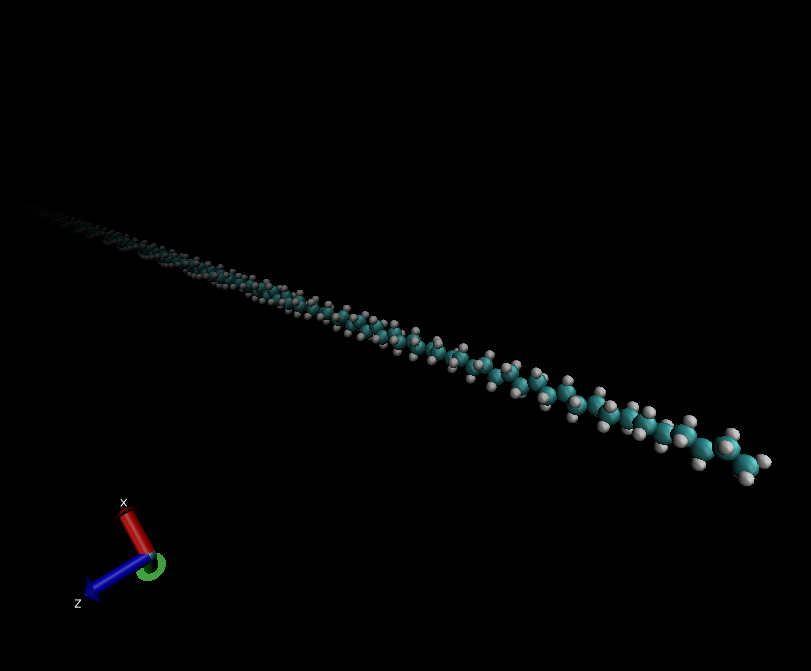
\includegraphics[width=0.48\textwidth]{figs/serial_geweke/VMD_serial_geweke_initial_geometry.png}
  \hfill
  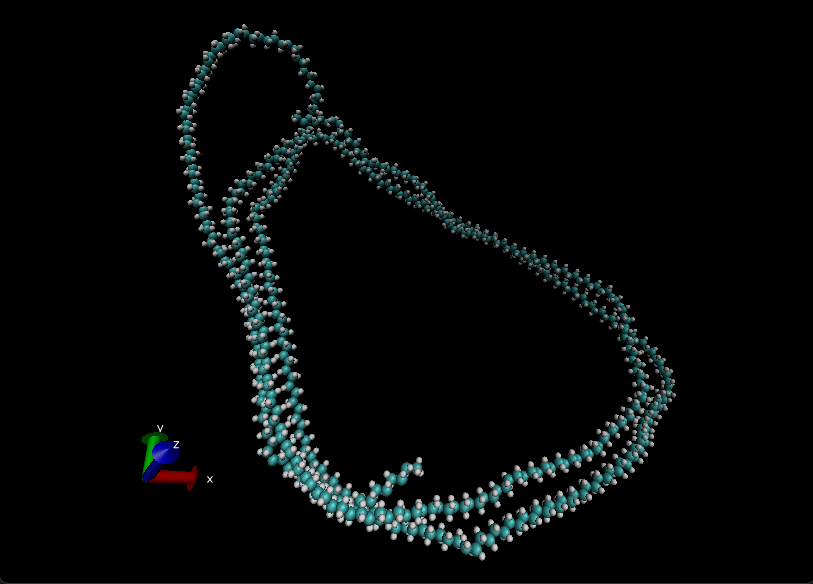
\includegraphics[width=0.48\textwidth]{figs/serial_geweke/VMD_serial_geweke_final_geometry.png}
  \caption{Left: initial configuration -- a nearly fully extended chain
    with all backbone carbons approximately collinear.
    Right: final production configuration -- a large open loop, 
    characteristic of a random-coil state.}
  \label{fig:vmd}
\end{figure}

The two VMD snapshots in Figure~\ref{fig:vmd} illustrate the scale of
the conformational change. The initial chain is nearly straight,
occupying roughly 650\,\AA\ end to end. The final structure is a
large folded loop with the two chain termini close together, far more
compact but not a dense collapsed globule.

\subsubsection{Structural Observables}

\begin{figure}[htbp]
  \centering
  
\includegraphics[width=0.8\textwidth]{figs/serial_geweke/observables_evolution_500_4_10000000_300.00.pdf}
  \caption{Radius of gyration $R_g$ (top) and end-to-end distance $R_{ee}$
    (bottom) across equilibration and production. The dashed vertical
    line marks the Geweke equilibration boundary at ${\approx}3.9 \times
    10^6$ steps.}
  \label{fig:observables}
\end{figure}

Figure~\ref{fig:observables} shows $R_g$ and $R_{ee}$ plotted
continuously across equilibration and production. $R_g$ begins at
approximately 185\,\AA\ and collapses to ${\approx}39$\,\AA\ within
the first 300\,000 steps, after which it fluctuates by only ${\sim}1$\,\AA\
around its mean for the remainder of the run. $R_{ee}$ follows a similar
rapid collapse from ${\approx}650$\,\AA\ to ${\approx}75$\,\AA, but
shows larger fluctuations in production (${\sim}15$\,\AA\ peak-to-peak),
which is expected: unlike $R_g$, which averages over all atoms, $R_{ee}$
depends only on the two terminal carbons and is therefore more sensitive
to large-scale rearrangements of the chain ends.

Both observables had converged well before the Geweke criterion declared
equilibrium at ${\approx}3.9 \times 10^6$ steps.

\subsubsection{Energy Evolution}

\begin{figure}[htbp]
  \centering
  
\includegraphics[width=0.8\textwidth]{figs/serial_geweke/energy_evolution_500_4_10000000_300.00.pdf}
  \caption{Total, Lennard-Jones, and torsional energy across
    equilibration and production. Dashed line marks the
    equilibration boundary.}
  \label{fig:energy}
\end{figure}

Figure~\ref{fig:energy} shows the three energy components. At step 1, the total energy is approximately 200\,kcal/mol, with the LJ term slightly negative around ---25\,kcal/mol (the extended chain has few close non-bonded contacts) and the torsional term near 230\,kcal/mol. Within the first million steps the chain folds rapidly, driving the LJ energy from ${\approx}{-25}$ to ${\approx}{-150}$\,kcal/mol as many atom pairs enter the attractive region of the LJ well simultaneously. The total energy settles to ${\approx}50$\,kcal/mol ($= {-150} + 200$\,kcal/mol from the two components). The torsional energy changes comparatively little (230 to 200\,kcal/mol), indicating that local torsional relaxation is much faster than global chain reorganization and that the initial configuration already had a broadly reasonable dihedral distribution.

After the equilibration boundary all three quantities fluctuate
stably, with no systematic drift visible over the full 10 million
production steps.

\subsubsection{Torsion Angle Distribution}

\begin{figure}[htbp]
  \centering
  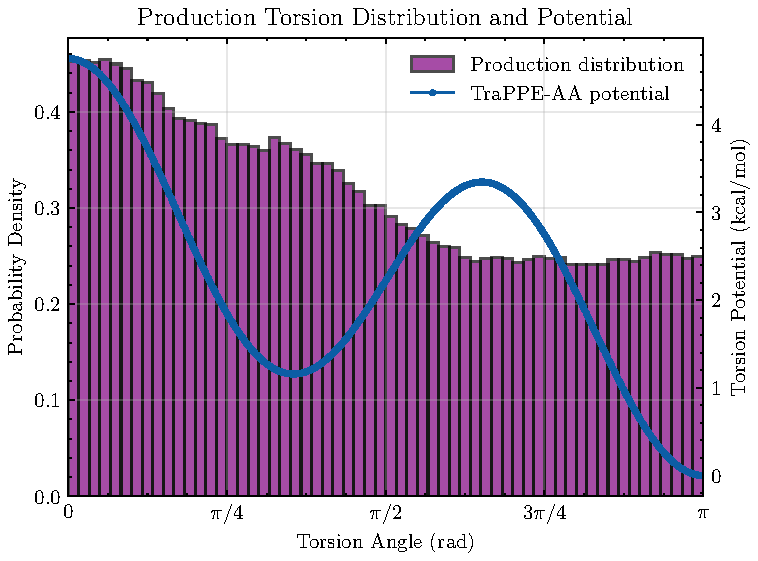
\includegraphics[width=0.8\textwidth]{figs/serial_geweke/torsion_distribution_500_4_10000000_300.00.pdf}
  \caption{Production-phase torsion angle distribution (purple
    histogram) overlaid with the OPLS-AA effective backbone potential
    (blue curve, right axis).}
  \label{fig:torsion}
\end{figure}

Figure~\ref{fig:torsion} shows the production torsion angle
distribution alongside the OPLS-AA effective backbone potential.
The histogram is concentrated almost entirely near $\phi = \pi$,
with the rest of the angular range essentially unoccupied. A small
gauche shoulder is visible near $\phi \approx \pi/3$, and the cis
region ($\phi \approx 0$) is absent from the distribution. This
population hierarchy is consistent with the potential: the global
minimum is at $\phi = \pi$ ($U = 0$), the gauche well sits
approximately 1.2\,kcal/mol above it, and the cis barrier reaches
approximately 4.7\,kcal/mol -- large relative to
$k_BT = 0.59$\,kcal/mol at 300\,K.

The equilibrium torsional energy of approximately 200\,kcal/mol
visible in Figure~\ref{fig:energy} is consistent with this
distribution. The torsional potential rises steeply from its
minimum at $\phi = \pi$, so small thermal fluctuations within
the trans well already carry a non-zero energy contribution per
dihedral. Summed across all backbone dihedrals, these
fluctuations account for the observed $E_{\mathrm{tors}}$ without
requiring significant population outside the trans region.

\subsection{Interpretation}

The simulation results are consistent with expected polymer behaviour
at 300\,K. The chain collapses from its initial extended geometry
within a few hundred thousand steps, after which it samples a
stationary conformational ensemble -- a compact random coil with
$R_g \approx 39$\,\AA\ and $R_{ee} \approx 75$\,\AA. These values
are substantially smaller than the fully extended length
(${\approx}650$\,\AA) but much larger than a fully collapsed globule
would give ($R_g \lesssim 15$\,\AA), confirming that the chain is in
a random-coil rather than a globular state.

The dominant contribution to energy stabilisation upon folding is
the Lennard-Jones term. In the extended configuration, most atom pairs
are beyond the LJ cutoff. As the chain folds, a large number of
non-bonded contacts accumulate in the attractive $r^{-6}$ region,
releasing ${\approx}125$\,kcal/mol of LJ energy. This is the
thermodynamic driving force for collapse at 300\,K.

The torsional distribution is governed by the total energy, not the
torsional term in isolation:
\begin{equation}
  E_{\mathrm{tot}} = E_{\mathrm{LJ}} + E_{\mathrm{tors}}.
\end{equation}
The Metropolis criterion accepts or rejects moves based on $\Delta E_{\mathrm{tot}}$.
Despite this coupling, the resulting torsional distribution is
dominated by the trans state in agreement with the
torsional potential hierarchy, because the torsional barriers are
large relative to $k_BT = 0.59$\,kcal/mol at 300\,K.

% Source ownership:
% - Itxaso

% ============================================================
\section{Cluster Compatibility}
\label{sec:cluster}
% ============================================================

Portability to shared HPC infrastructure required two targeted modifications.
First, the \texttt{Makefile} replaces the Fortran 2008 \texttt{open(newunit=u)}
syntax with explicit unit-number declarations compatible with Fortran 90
compilers available on the CERQT2 cluster. Second, a submission script
\texttt{1.run.sh} was created to load the appropriate GCC and OpenMPI modules
before compilation and execution. The \texttt{parameters.f90} file was adapted
to restore the \texttt{\#ifdef} preprocessor block controlling the
\texttt{explicit\_h} compilation flag, and a comment was added to the
\texttt{Makefile} explaining why the \texttt{-I\$(MPI\_INC\_DIR)} flag is
conditionally omitted in certain build configurations.

% ============================================================
% Source ownership:
% - Itxaso

% ============================================================
\section{MPI Parallelization: Independent Replicas}
\label{sec:parallel_replicas}
% ============================================================

\subsection{Justification}

The MPI parallelization implemented here is based on independent replica parallelism as a first step, while the energy evaluation and the Monte Carlo kernel can be parallelized subsequently (see the Energy Evaluation and Monte Carlo sections). First, independent replicas do not require inter-process communication inside the Monte Carlo loop, which keeps synchronization overhead very low. Second, running several initial configurations simultaneously makes it possible to assess how sensitive the final sampled ensemble is to the choice of starting geometry.

\subsection{Implementation: \texttt{main\_parallel\_replicas.f90}}

Starting from \texttt{main\_serial.f90}, three MPI ranks are launched
simultaneously. Each rank runs the identical Monte Carlo protocol (same
thermodynamic parameters, same number of steps) but is assigned a distinct
initial configuration and a perturbed random seed:

\begin{lstlisting}[caption={Rank-dependent configuration and seed assignment.}]
! MPI initialization
call MPI_Init(ierr)
call MPI_Comm_rank(MPI_COMM_WORLD, rank, ierr)
call MPI_Comm_size(MPI_COMM_WORLD, n_ranks, ierr)

! Assign initial configuration based on rank
select case (rank)
  case (0); conf_type = 1   ! all-trans (extended)
  case (1); conf_type = 4   ! helix / spring
  case (2); conf_type = 5   ! perturbed trans
end select

! Perturb the RNG seed so trajectories immediately diverge
rng_seed = rng_seed + rank * 104729

! Build the initial configuration and run the full MC protocol
call build_initial_conf(n_carbons, conf_type, explicit_h, coords, symbols)
call mc_run(...)

! Rank-labelled output so files do not overwrite each other
write(label, '(A,I1)') trim(base_label)//'_rank', rank
call write_trajectory(label, coords, symbols, n_atoms)
\end{lstlisting}

The three configurations chosen (\texttt{conf\_type} 1, 4, and 5) cover the
near-trans region from three distinct but close starting points: fully
extended, helical, and slightly perturbed extended. This choice maximises the
geometric diversity of the initial ensemble while keeping all replicas in
a physically reasonable region of conformational space.

A serial counterpart, \texttt{main\_serial\_replicas.f90}, runs the same
three configurations sequentially to provide a controlled performance
reference. Both versions employ wall-clock timing: \texttt{MPI\_Wtime} in the
parallel driver and an equivalent system-clock call in the serial one,
ensuring that the speedup ratios reported in Section~\ref{sec:scaling} reflect
actual elapsed time rather than CPU time.

\subsection{Discarded Parallelization: XYZ Trajectory Writing}

A second parallelization direction was explored: distributing the XYZ
trajectory write step across ranks, so that each rank writes its own frame
independently. The resulting wall-clock improvement was marginal (less than
2\% of total runtime), confirming that trajectory I/O is not the computational
bottleneck. The dominant cost lies in the energy evaluation and
Metropolis acceptance/rejection logic, as expected from the
$\mathcal{O}(N^2)$ Lennard-Jones loop. This branch was therefore discarded
and the simpler rank-labelled sequential write was kept.

% ============================================================
% Source ownership:
% - Itxaso

% ============================================================
\section{MPI Parallelization: Observable Post-Processing}
\label{sec:parallel_observables}
% ============================================================

\subsection{Design and Implementation}

Post-processing of the trajectory data has been parallelized in
\texttt{main\_parallel\_observables.f90}. Rather than decomposing a single
trajectory into contiguous frame blocks, the implementation operates at the
file level: all trajectory files are first enumerated in a manifest, rank 0
reads this manifest, and the complete file list is broadcast to all MPI ranks.
Each rank then processes a round-robin subset of trajectory files,
independently computing the radius of gyration \(R_g\), the end-to-end
distance \(R_{ee}\), and the torsional statistics for the configurations
assigned to it.

This design was chosen because the available data are naturally distributed
across multiple trajectory files, corresponding to different configuration
types and simulation phases (\texttt{equil} and \texttt{prod}). A file-level
distribution avoids repeated file seeks inside large XYZ trajectories, keeps
the implementation simple, and preserves a fully embarrassingly parallel local
workload. At the same time, it remains fully compatible with collective MPI
communication for global aggregation.

A first collective step is performed through \texttt{MPI\_Bcast}, which is used
to distribute the manifest and the maximum number of torsional degrees of
freedom to all ranks. After each rank has completed its local file subset, a
mid-run checkpoint is evaluated by means of \texttt{MPI\_Allreduce}. In this
step, the partial frame counts and partial \(R_g\) sums are synchronised across
all processes, so that the global partial mean can be computed before the final
aggregation stage. This checkpoint was introduced as a lightweight example of
active communication during the computation phase, beyond the final collection
of results.

\begin{lstlisting}[caption={Round-robin file distribution and MPI checkpoint in \texttt{main\_parallel\_observables.f90}.}]
! Each rank processes a round-robin subset of trajectory files
do ifile = rank + 1, nfiles, num_procs
  call process_trajectory(trim(files(ifile)), max_phi, &
       local_file_count, local_frame_count, &
       local_sum_rg, local_sum_rg2, local_sum_ree, local_sum_ree2, &
       local_nphi, local_sum_phi, local_sum_phi2)
enddo

! Mid-run checkpoint: all ranks obtain the global partial mean of Rg
call MPI_Allreduce(local_frame_count, ckpt_frame_count, n_conf*n_phase, &
                   MPI_INTEGER, MPI_SUM, MPI_COMM_WORLD, ierr)
call MPI_Allreduce(local_sum_rg, ckpt_sum_rg, n_conf*n_phase, &
                   MPI_DOUBLE_PRECISION, MPI_SUM, MPI_COMM_WORLD, ierr)

! Final aggregation on rank 0
call MPI_Reduce(local_sum_rg, global_sum_rg, n_conf*n_phase, &
                MPI_DOUBLE_PRECISION, MPI_SUM, 0, MPI_COMM_WORLD, ierr)
\end{lstlisting}

The final global statistics are obtained on rank 0 through a series of
\texttt{MPI\_Reduce} operations, which combine the local sums, squared sums,
frame counts, and torsional accumulators into global averages and standard
deviations. The corresponding summary files
(\texttt{summary\_global\_np1.dat}, \texttt{summary\_global\_np2.dat},
\texttt{summary\_global\_np4.dat}, and \texttt{summary\_global\_np8.dat}) show
that the numerical results are identical for all tested values of \(n_p\),
confirming that the parallelization preserves the observable averages exactly.

The benchmark driver is invoked from the cluster submission script
\texttt{3.run\_parallel\_observables\_np.sh}, which executes the same
post-processing workflow for \(n_p \in \{1,2,4,8\}\), records both MPI and
shell wall-clock times, and writes per-process summary files for subsequent
comparison.

% ============================================================
% Source ownership:
% - Manel: collaborative equilibration, Boltzmann roulette, metrics
% - Arthur: ensemble averaging / orchestrator narrative
% - Itxaso: MUST add "Orchestrator Initial Config Read & Broadcast"

\section{MPI Parallelization: Collaborative Equilibration}
\label{sec:mpi_collab}

\subsection{Orchestrator Initial Configuration Read and Broadcast}

In the MPI version of the program, rank 0 acts as the central
orchestrator. Its role is to read the initial configuration files,
decide whether each conformation must still be equilibrated or can
directly enter production, and distribute the corresponding work to the
workers.

At startup, the master reads the input settings and the geometry
required to initialise each polymer configuration. If an equilibrated
geometry is already available for a given configuration, the program can
bypass the equilibration stage and directly unlock the corresponding
production replicas. Otherwise, the master marks that configuration as
pending collaborative equilibration.

For configurations that still require equilibration, rank 0 assigns a
group of workers to the same initial structure. These workers all begin
from the same geometry, but each one uses a different random seed so
their trajectories immediately diverge. The master therefore provides a
common starting point while still allowing independent exploration of
phase space.

This orchestrator stage also centralises the campaign-level file
handling. Workers do not need to parse the full simulation manifest or
determine which configurations are ready for production. Instead, they
receive either the job descriptor or the coordinates required for the
task they have been assigned, initialise their local arrays, and begin
Monte Carlo propagation.

\subsection{Equilibration Optimization}

Rather than assigning a single worker to equilibrate each configuration
type independently, a group of \texttt{workers\_per\_equil} MPI workers
is assigned to each configuration type simultaneously. Each worker
starts from the same initial geometry but with a different random seed,
for example \texttt{rngseed = rank * 104729}, ensuring that trajectories
immediately diverge and explore distinct regions of conformational
space.

Every \texttt{sync\_interval} Monte Carlo steps, a synchronisation
protocol is executed. Each worker sends its current energy and
\(R_g\) to the master, which selects the most representative
configuration via a Boltzmann-weighted roulette wheel and broadcasts
those coordinates back to the non-winning workers in the group. The
winning worker continues its trajectory uninterrupted, preserving the
best conformational path found so far.

The purpose of this strategy is to reduce the time required to reach a
well-equilibrated low-energy configuration. Instead of waiting for one
trajectory to escape a poor metastable region on its own, the algorithm
lets several replicas search in parallel and periodically shares the
best result across the group. In this way, all workers benefit from the
progress made by the most successful replica.

\subsection{Replica Selection: Boltzmann Roulette Wheel}

At each synchronisation point, the master assigns a statistical weight
to each replica \(i\) based on its total energy \(E_i\):
\[
w_i = \exp\!\left(-\frac{E_i - E_{\min}}{k_B T_{\mathrm{virt}}}\right),
\]
where \(E_{\min}\) is the lowest energy in the current group and
\(T_{\mathrm{virt}}\) is a virtual temperature.

The virtual temperature is a purely algorithmic parameter with no
physical meaning. It controls how aggressively low-energy replicas are
favoured:
\begin{itemize}
\item \(T_{\mathrm{virt}} \to 0\): deterministic selection of the
minimum-energy replica.
\item \(T_{\mathrm{virt}} \to \infty\): uniform selection, ignoring
energies.
\end{itemize}

A uniform random number then samples this distribution via roulette-wheel
selection. The selected replica becomes the winner of that
synchronisation round, and its coordinates are sent to the non-winning
workers so they can resume the search from the most promising state
found so far.

\subsection{MPI Communication Protocol}

The synchronisation uses only point-to-point MPI operations
\texttt{MPI\_Send} and \texttt{MPI\_Recv} to avoid the need for
temporary communicators or collective operations across worker
subgroups. At each sync point, the master loops over all workers in the
active equilibration group and performs the following exchanges.

\begin{table}[h!]
\centering
\begin{tabular}{clll}
\toprule
Step & Direction & Tag & Content \\
\midrule
1 & worker \(\rightarrow\) master & \texttt{TAG\_SYNC\_OBS} &
\(E_{\mathrm{tot}}, R_g^2\) \\
2 & master \(\rightarrow\) worker & \texttt{TAG\_SYNC\_CTRL} &
control signal, \texttt{bestlocalidx} \\
3 & worker \(\rightarrow\) master & \texttt{TAG\_EQUIL\_COORDS} &
full coordinate array \\
4 & master \(\rightarrow\) non-winners & \texttt{TAG\_SYNC\_COORDS} &
winning coordinates \\
\bottomrule
\end{tabular}
\caption{Point-to-point synchronisation protocol used during collaborative equilibration.}
\end{table}

Once the Geweke test declares equilibrium, the master saves the
equilibrated geometry to \texttt{../results/equilibrated\_cX.xyz} and
unlocks the 10 production jobs for that configuration type in the task
queue.

\subsection{Metrics and Methodology}

This section evaluates the performance of the equilibration
optimization technique compared to the serial baseline. The system
studied is configuration 1, a chain of 500 carbons at \(T = 300\) K
including hydrogens. Efficiency is evaluated based on the time to reach
specific energy thresholds \(E_{\mathrm{tot}} = 110\), 100, and
90 kcal/mol.

The speedup is defined as
\[
S_w = \frac{\mathrm{Steps}_{\mathrm{serial}}}
           {\mathrm{Steps}_{\mathrm{parallel},\,w}},
\]
where \(w\) is the number of workers participating in the collaborative
equilibration group. Efficiency is then defined as
\[
\eta_w = \frac{S_w}{w}.
\]

The table below summarises the number of MC steps required by different
worker configurations to reach the target energy levels.

\begin{table}[h!]
\centering
\begin{tabular}{ccccc}
\toprule
Threshold & Workers \(w\) & Steps Required & Speedup \(S_w\) & Efficiency \(S_w / w\) \\
\midrule
110 kcal/mol & 1 & 590,000  & 1.00  & 1.00 \\
110 kcal/mol & 2 & 70,000   & 8.43  & 4.21 \\
110 kcal/mol & 4 & 140,000  & 4.21  & 1.05 \\
110 kcal/mol & 8 & 50,000   & 11.80 & 1.47 \\
\midrule
100 kcal/mol & 1 & 1,180,000 & 1.00  & 1.00 \\
100 kcal/mol & 2 & 350,000   & 3.37  & 1.68 \\
100 kcal/mol & 4 & 210,000   & 5.62  & 1.40 \\
100 kcal/mol & 8 & 50,000    & 23.60 & 2.95 \\
\midrule
90 kcal/mol & 1 & 2,400,000 & 1.00  & 1.00 \\
90 kcal/mol & 2 & 1,780,000 & 1.35  & 0.67 \\
90 kcal/mol & 4 & 570,000   & 4.21  & 1.05 \\
90 kcal/mol & 8 & 160,000   & 15.00 & 1.87 \\
\bottomrule
\end{tabular}
\caption{Monte Carlo steps required to reach selected energy thresholds during collaborative equilibration.}
\end{table}

These results show that the method can exhibit superlinear speedup.
This is not just because more workers are used, but because the search
itself changes. A population of replicas explores several
conformational regions at once, and once one replica finds a much
better basin, that discovery is broadcast to the others at the next
synchronisation point.

For this reason, the observed acceleration is partly computational and
partly algorithmic. The collaborative protocol does not simply divide
the same work among more processes; it improves the probability of
finding favourable states earlier than a single serial trajectory would.

\begin{figure}[h!]
  \centering
  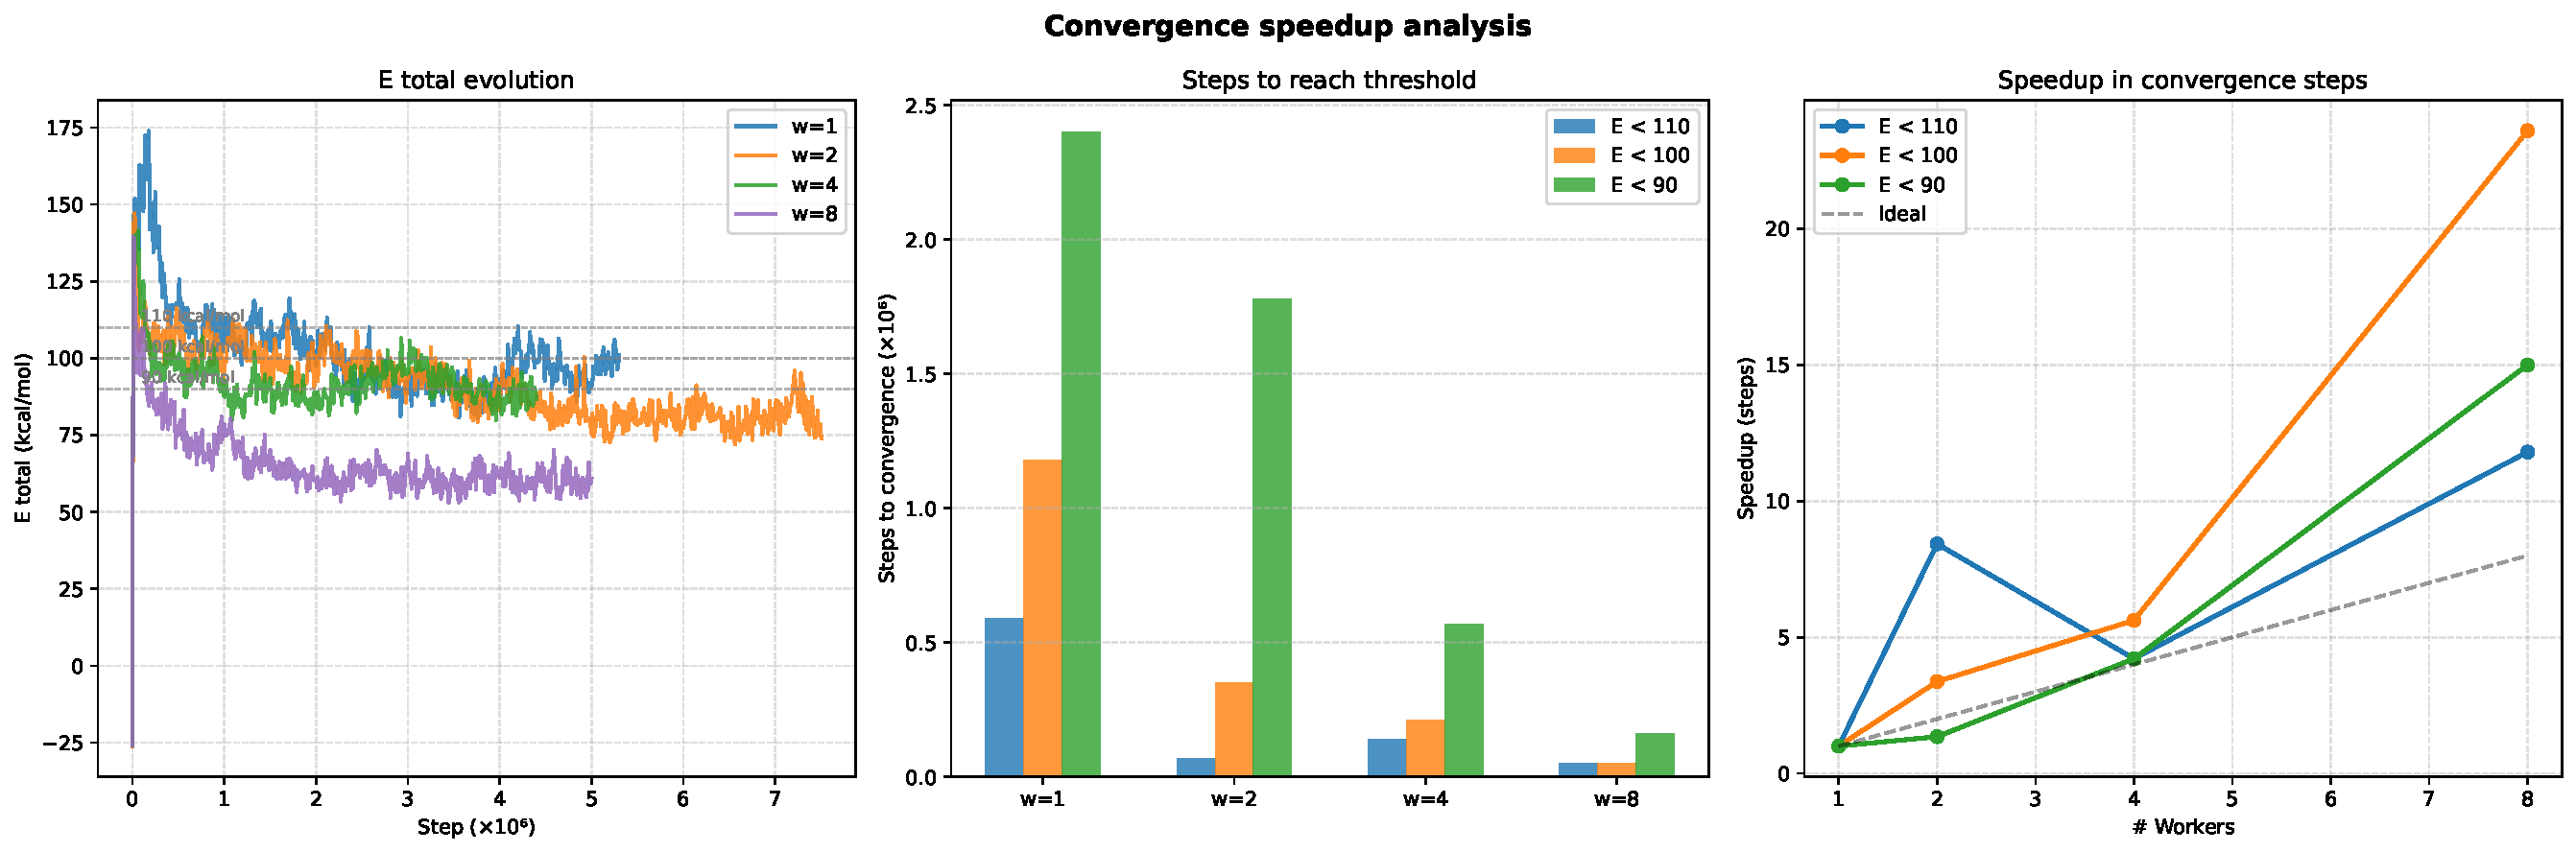
\includegraphics[width=\textwidth]{convergence_speedup_equil.pdf}
  \caption{Convergence speedup analysis for collaborative equilibration.}
\end{figure}

\subsection{Ensemble Averaging and Star Topology}

Once an equilibrated geometry has been found, the workflow switches from
collaborative equilibration to large-scale production sampling. At this
stage, rank 0 acts as a central dispatcher in a star-topology MPI
scheme, while the remaining ranks behave as workers that repeatedly
request new tasks from the master.

The master maintains a global queue of production jobs. Each job
corresponds to an independent production replica, and workers are
assigned new jobs dynamically as soon as they finish their current one.
This avoids the load imbalance that would appear if all replicas were
distributed statically at launch, since individual trajectories may
still differ slightly in runtime.

The dispatcher listens using a tag-based communication pattern and can
react to whichever worker becomes free first. In practice, this means
that workers request work, receive a production assignment, run the
simulation, write their outputs, and notify the master when they have
finished. The master then either sends another job or terminates the
worker once the queue has been exhausted.

This star-topology design turns the MPI layer into an ensemble averaging
engine. Independent production replicas are generated as efficiently as
possible, and the final observables are obtained by averaging over the
outputs of all completed runs. In this phase, the objective is no
longer to accelerate the equilibration of a single chain, but to
maximize statistical throughput across the whole ensemble.

\begin{table}[h!]
\centering
\begin{tabular}{cll}
\toprule
Direction & Tag & Meaning \\
\midrule
worker \(\rightarrow\) master & \texttt{TAG\_REQUEST\_WORK} & worker requests a new task \\
master \(\rightarrow\) worker & \texttt{TAG\_DO\_PROD} & start a production replica \\
master \(\rightarrow\) worker & \texttt{TAG\_WAIT} & remain idle temporarily \\
master \(\rightarrow\) worker & \texttt{TAG\_DIE} & terminate execution \\
worker \(\rightarrow\) master & \texttt{TAG\_PROD\_DONE} & production replica finished \\
\bottomrule
\end{tabular}
\caption{Tag-based work distribution in the star-topology production phase.}
\end{table}

\begin{figure}[h!]
  \centering
  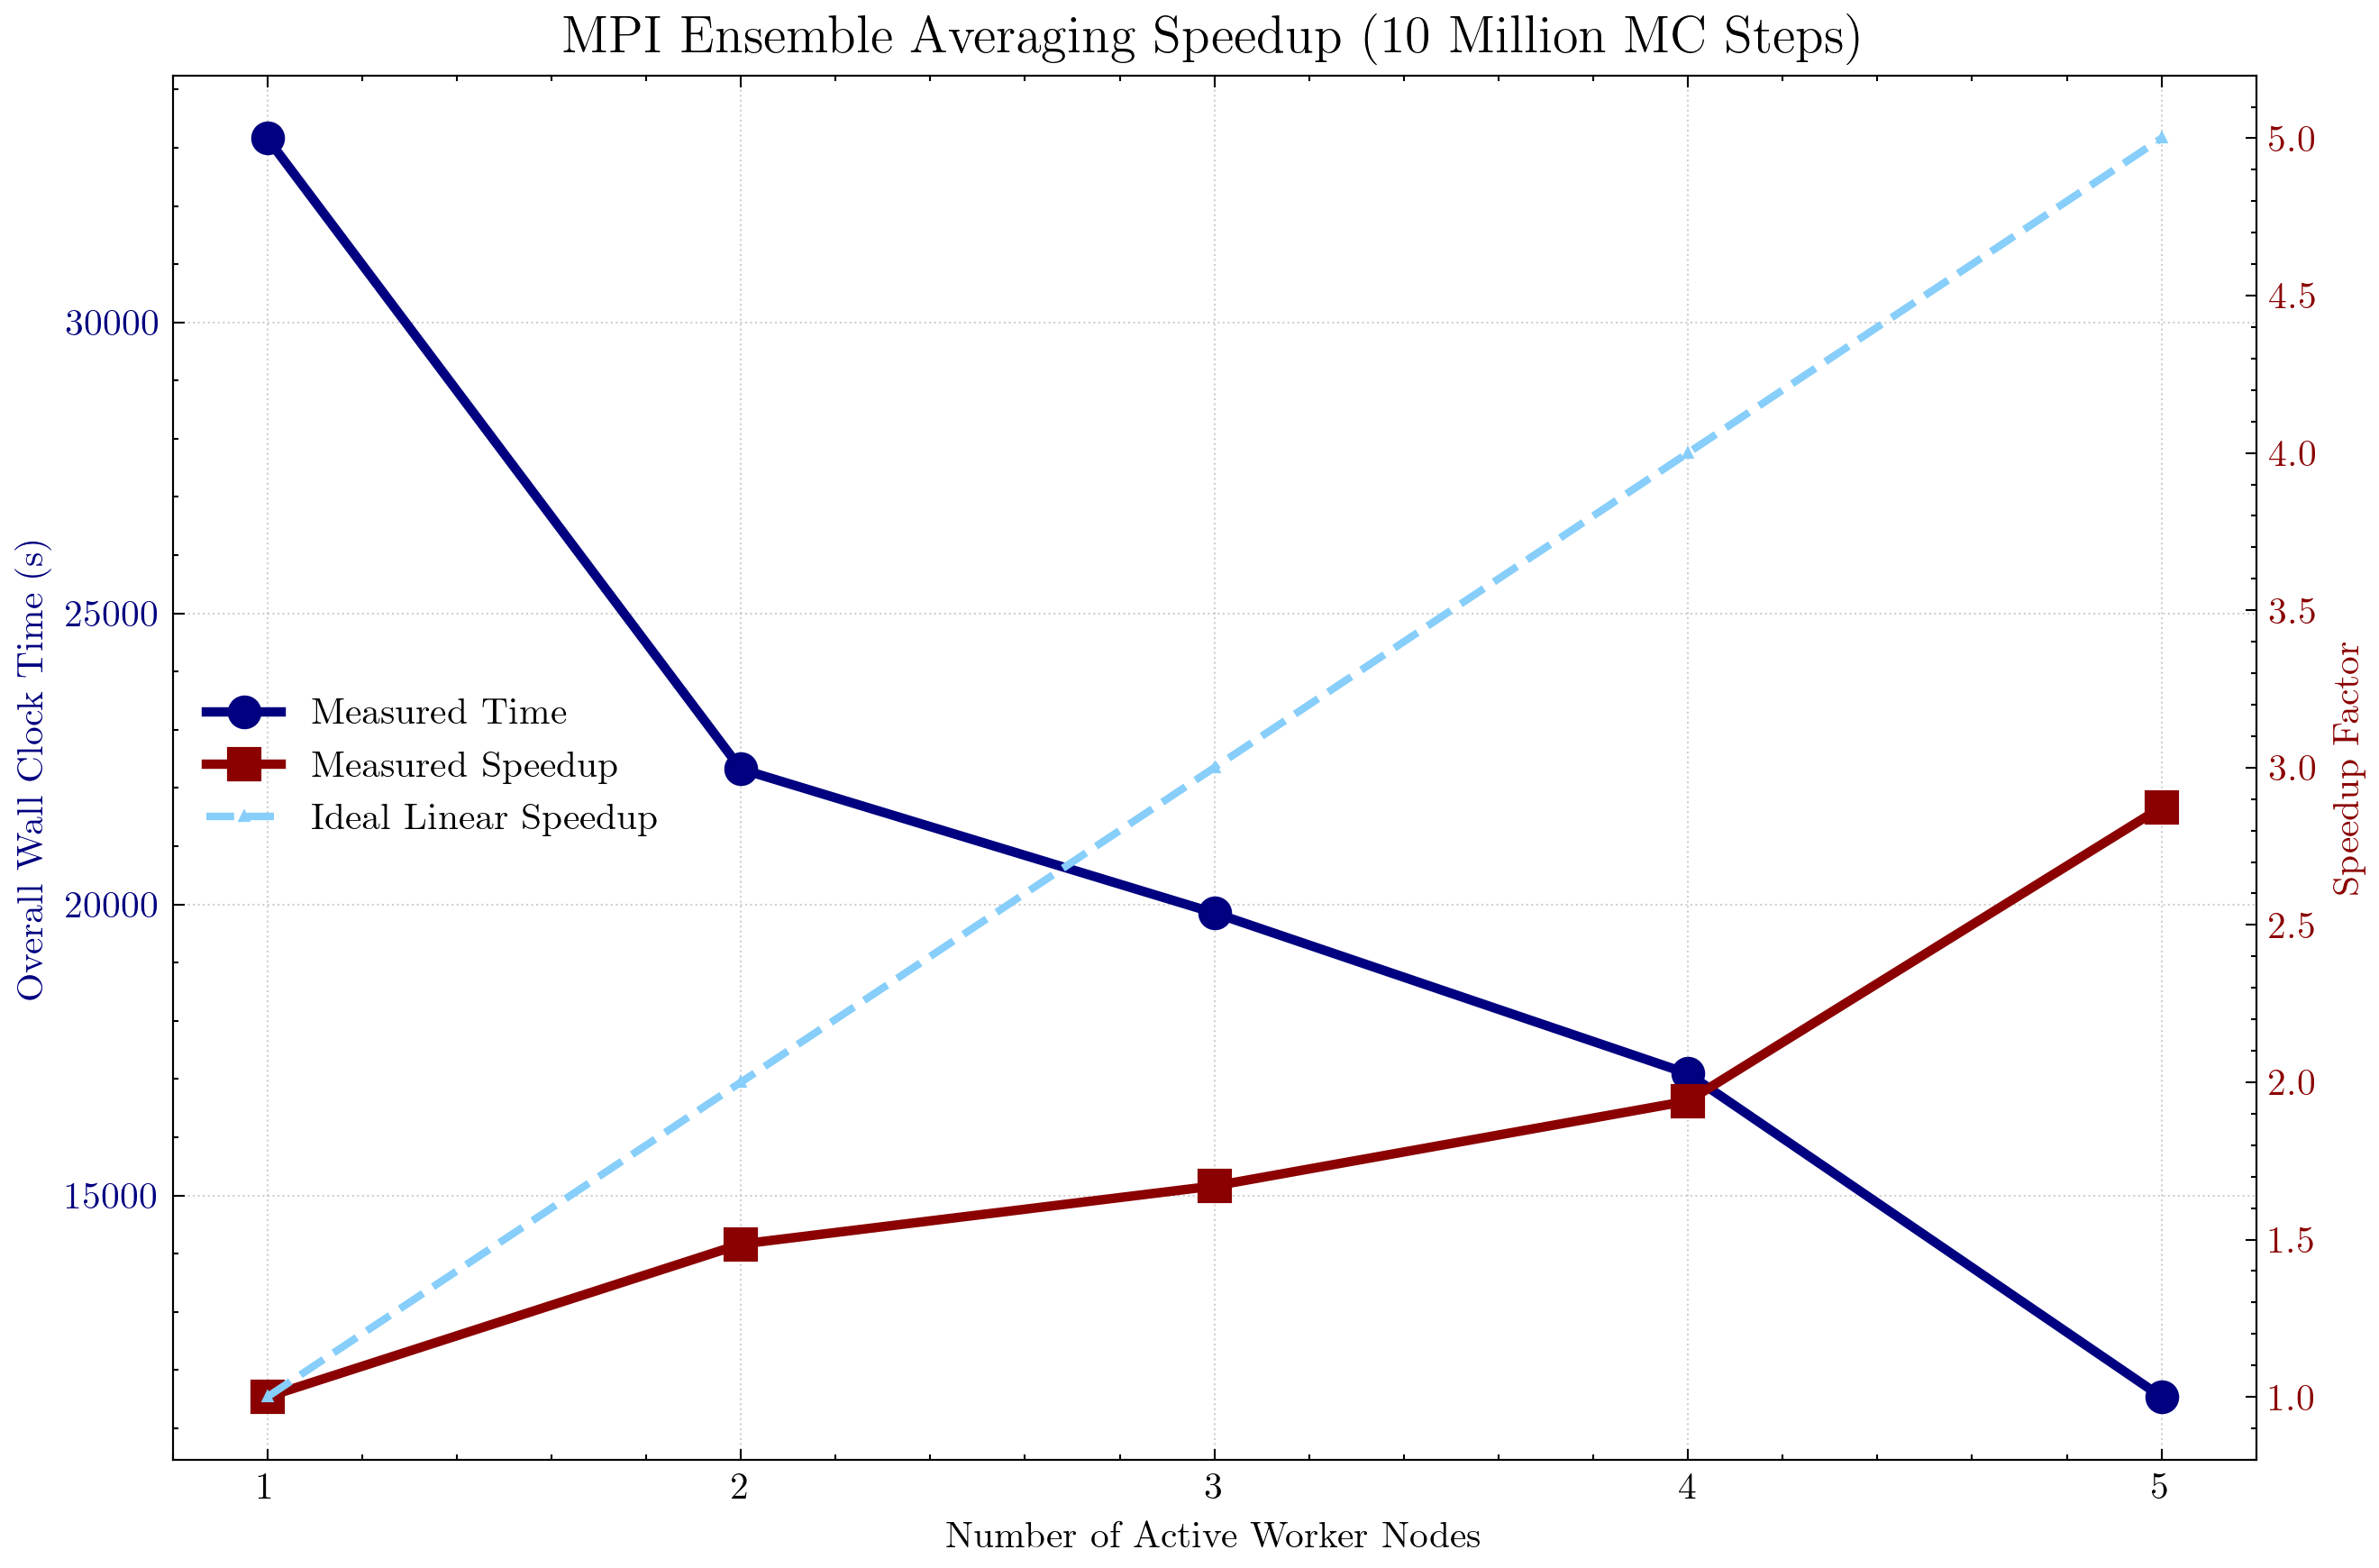
\includegraphics[width=\textwidth]{parallel_star_speedup_plot.png}
  \caption{Timing and efficiency of the orchestrator-worker production workflow.}
\end{figure}
% Source ownership:
% - Mainly Arthur/Manel/Oliwier
% - pending final benchmark figures / commentary

\section{OpenMP Parallelization}
\label{sec:openmp}

\subsection{\texttt{compute\_total\_energy}}

The dominant cost in \texttt{compute\_total\_energy} is the
\(O(N^2)\) double loop over non-bonded Lennard-Jones pairs. Each
iteration is independent --- it reads a pair of coordinates, evaluates
\texttt{ljpairenergy}, and adds to a running sum --- which makes it a
natural fit for OpenMP worksharing.

The outer loop is distributed across threads with
\texttt{!\$omp parallel do}, with the inner index, the squared
distance \(r^2\), and the dihedral cosine \texttt{cosphi} declared
\texttt{private} to prevent cross-thread interference. The global
accumulators \texttt{elj} and \texttt{etors} are aggregated safely
using a \texttt{reduction(+:...)} clause.

The two loops inside the subroutine have different iteration structures
and were scheduled accordingly. The LJ pair loop has a triangular
iteration space because the inner bound depends on the outer index, so
\texttt{schedule(dynamic,10)} is used to prevent faster threads from
sitting idle while slower ones finish larger chunks of work. The
torsional loop over the carbon backbone is uniform in length and uses
the default static scheduling, which has lower overhead when the
workload is balanced.

Both parallel regions are wrapped in an \texttt{if(omp\_totalenergy)}
runtime guard, which is set from the input file. This allows the same
binary to run in purely serial mode during development or lightweight
tests without any code changes.

\subsection{\texttt{delta\_energy}}

The \texttt{delta\_energy} subroutine is the true bottleneck of the MC
loop --- it is called once per accepted or rejected move, millions of
times per simulation. The key algorithmic feature here is the dynamic
partitioning of atoms into \texttt{fixedlist} and \texttt{movedlist} at
the start of each call.

Only cross-interactions between fixed and moved atoms can have changed
during a pivot, so the LJ loop processes exclusively those pairs rather
than the full \(O(N^2)\) set. This drastically reduces the amount of
work required for a local move and makes the subroutine much more
sensitive to efficient parallelization.

The two nested loops over fixed and moved form a perfectly rectangular
iteration space, which makes \texttt{collapse(2)} effective: it merges
both loops into a single flat range of \(n_{\mathrm{fixed}}
n_{\mathrm{moved}}\) iterations and distributes them evenly across
threads.

Since pivot moves near the ends of the chain move very few atoms,
spawning threads for only a small number of pairs would cost more than
it saves. The parallel block is therefore gated by
\texttt{if(omp\_deltaenergy .and. nfixed*nmoved > 1000)}, ensuring that
OpenMP is only activated when the workload genuinely justifies the
threading overhead.

\subsection{Benchmarking Methodology}

To quantify the effect of thread count on both energy routines, a
dedicated benchmark program \texttt{mainbenchtotal.f90} was written. It
performs 10,000 back-to-back calls to
\texttt{compute\_total\_energy} for a given chain size and reports the
wall time via \texttt{MPI\_Wtime}.

Two shell scripts automate the full benchmark sweeps.
\texttt{4.runomptotaltest.sh} compiles and runs the benchmark binary
across thread counts of 1, 2, 3, and 4 for chain sizes of 20, 50, 100,
and 500 carbons, writing the results to a CSV file in the benchmark
results folder.

\texttt{5.runompdeltatest.sh} follows the same structure but targets
\texttt{delta\_energy} by running full 1M-step MC simulations via
\texttt{mainparallelreplicas.x} and extracting wall time from the CPU
output files. Both scripts are written for the cluster queue and load
the appropriate MPI module.

The results are plotted by \texttt{plotbenchmarks.py}, which reads both
CSV files and produces per-chain-size scaling plots as PDF figures.

A note must be made regarding the \texttt{delta\_energy} benchmark:
because it is measured inside full Monte Carlo production runs, the
timings are affected by randomness. Different random trajectories lead
to different accepted moves and different moved/fixed partitions, so the
workload is not bitwise identical between runs. For that reason, the
\texttt{delta\_energy} benchmark should be interpreted as a practical
end-to-end timing measurement rather than as a perfectly controlled
microbenchmark.

% Oliwier to add images / results / analysis

\subsection{SIMD Exploration}

An attempt was made to additionally exploit single-core SIMD
vectorization on the \texttt{ljpairenergy} function using the
\texttt{!\$omp declare simd} directive. The idea was to generate a
vectorized variant of the function callable from an
\texttt{!\$omp simd}-annotated inner loop, allowing each thread to
process multiple atom pairs simultaneously using AVX registers.

In practice, activating this required structural changes to
\texttt{delta\_energy} that conflicted with the existing threading
design. The \texttt{collapse(2)} clause and the inner-loop
\texttt{cycle} on \texttt{isexcluded} are not naturally compatible with
SIMD regions, and removing them in order to support vectorization
degraded the thread load balancing that \texttt{collapse(2)} provides.

Given that OpenMP threading was the primary parallelization goal, the
SIMD experiment was abandoned and the directive was removed from the
code. It remains a direction worth revisiting, particularly if the pair
loops are later refactored to use pre-filtered pair lists that eliminate
the exclusion branch entirely.
% Source ownership:
% - Itxaso: scaling of replicas + observables
% - Arthur/Manel: broader discussion and combined-program logic

\section{Scaling Analysis and Discussion}
\label{sec:scaling}

\subsection{Replica Parallelism: Speedup vs. System Size and Run Length}

The independent-replica MPI strategy was benchmarked by varying both the
polymer size and the production run length. In this approach, each MPI
worker executes a different production replica, so the total wall time
depends primarily on how much useful work can be distributed across
workers before communication and orchestration overhead begin to matter.

The first scaling study varies the number of carbons while keeping the
simulation length fixed. As the chain becomes larger, each replica
contains more internal work, especially in the energy calculations and
observable evaluations, so the MPI orchestration overhead becomes less
significant relative to the total runtime. For this reason, larger
systems are expected to display better parallel efficiency than very
small ones.

The second study varies the number of Monte Carlo steps for a fixed
system size. Short runs do not amortize the startup, scheduling, and I/O
costs very well, whereas longer runs allow each worker to spend a much
greater fraction of time performing actual MC sampling. Consequently,
speedup generally improves as the number of production steps increases.

In both cases, the speedup is not expected to be perfectly linear. The
master node still performs administrative tasks such as initial file
reading, dispatching jobs, receiving completion messages, and managing
the production queue. This means that part of the total hardware budget
is always reserved for orchestration rather than direct numerical work.

\begin{figure}[h!]
  \centering
  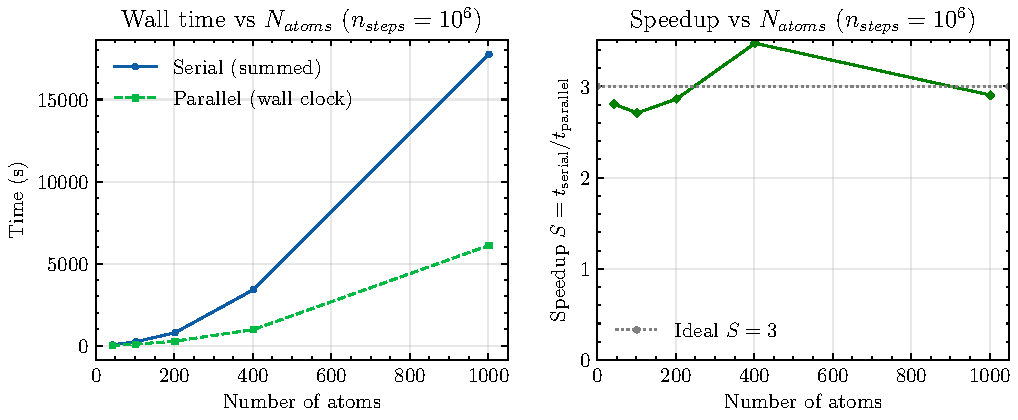
\includegraphics[width=\textwidth]{speedup_vs_natoms.pdf}
  \caption{Speedup of independent-replica parallelization: speedup as a function of chain length
           (\(N_C \in \{20,50,100,200,500\}\), \(n_{\text{steps}} = 10^6\)).
           All runs use 3 MPI ranks. The dashed line indicates ideal
           linear scaling (\(S = 3\)).}
\end{figure}

\begin{figure}[h!]
  \centering
  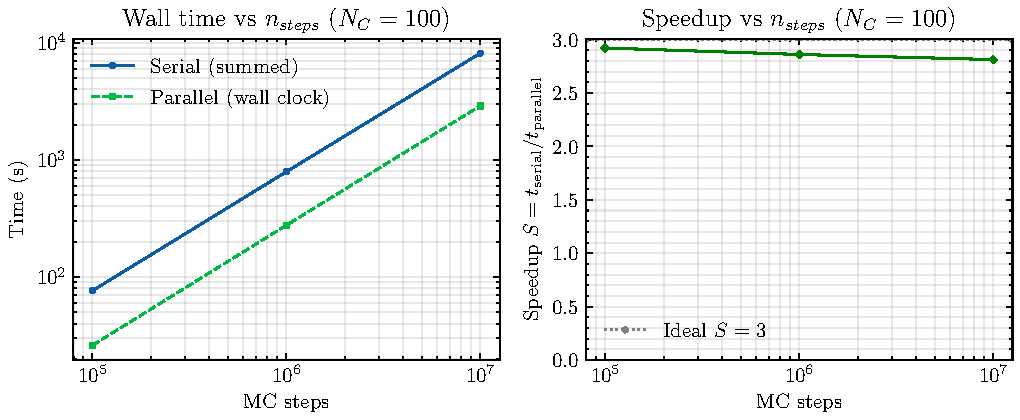
\includegraphics[width=\textwidth]{speedup_vs_nsteps.pdf}
  \caption{Speedup of independent-replica parallelization: speedup as a function of run length
           (\(n_{\text{steps}} \in \{10^5, 10^6, 10^7\}\), \(N_C = 100\)).
           All runs use 3 MPI ranks. The dashed line indicates ideal
           linear scaling (\(S = 3\)).}
\end{figure}

\subsection{Observable Post-Processing: Strong Scaling}

A second scaling study was carried out for the observable
post-processing kernel, implemented in
\texttt{main\_parallel\_observables}. Unlike the production simulations,
this stage is a strong-scaling problem: the total dataset is fixed, and
the number of MPI processes is increased to measure how efficiently the
same workload can be completed.

Each process reads a subset of trajectory files, computes the radius of
gyration, end-to-end distance, and torsional statistics, and
accumulates local partial sums. At the end of the run, the global
results are assembled through MPI reductions on rank 0, which writes the
final averaged observables.

This workload is well suited to MPI because each trajectory file can be
processed independently for most of the runtime. Communication is only
required at the end, when the local statistics are combined into a
single global dataset. As a result, the observable analysis behaves much
closer to an embarrassingly parallel workload than the simulation phase
itself.

The scaling is therefore expected to be strong for moderate process
counts, with efficiency gradually decreasing once the number of workers
becomes large compared to the number of files. At that point, the amount
of useful work per process shrinks and the fixed costs of process launch,
file I/O, and final reductions become more visible.

\begin{figure}[h!]
  \centering
  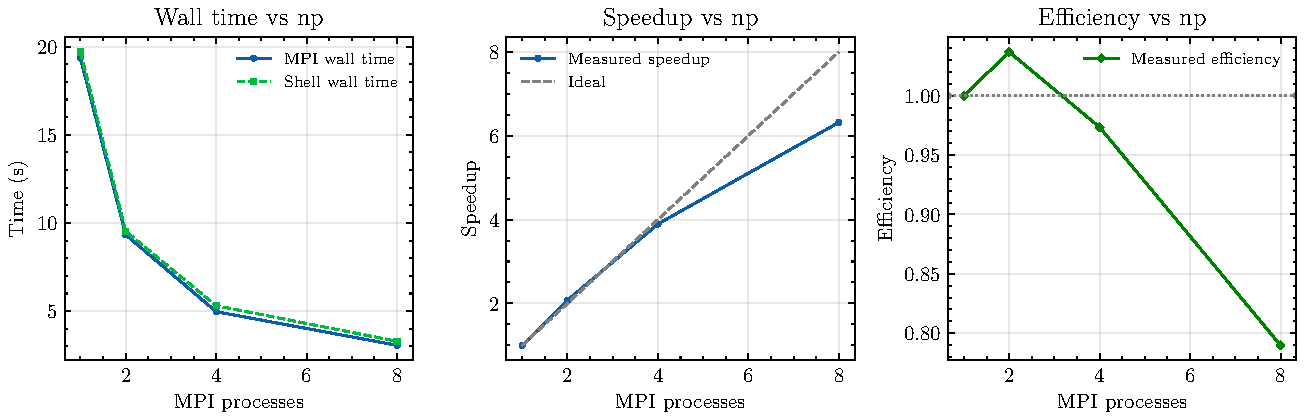
\includegraphics[width=\textwidth]{benchmark_vs_np.pdf}
  \caption{Strong scaling of the observable post-processing kernel.
           MPI wall-clock time (solid circles) and shell-measured
           elapsed time (dashed squares) as a function of the number of
           MPI processes \(n_p\).}
\end{figure}

\begin{figure}[h!]
  \centering
  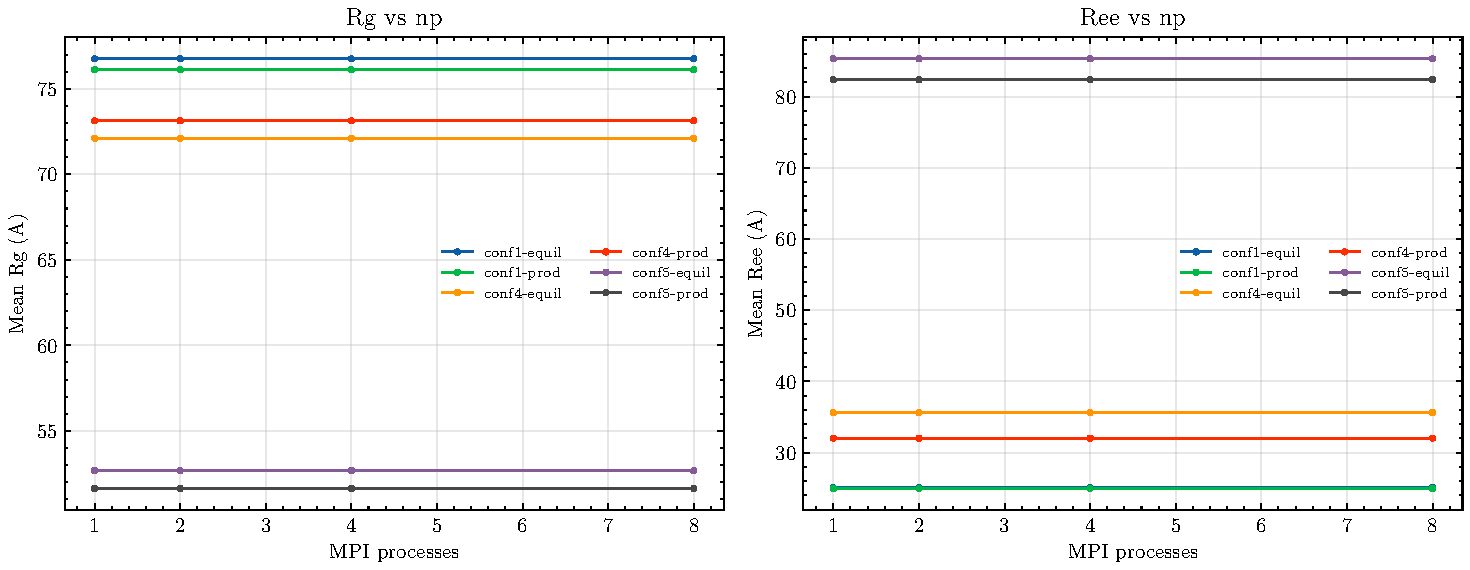
\includegraphics[width=\textwidth]{observables_vs_np.pdf}
  \caption{Mean radius of gyration \(R_g\) and mean end-to-end distance
           \(R_{ee}\) as a function of the number of MPI processes \(n_p\).
           The overlap of all curves confirms that the observable averages are
           preserved exactly across the tested parallel decompositions.}
\end{figure}

\subsection{Discussion}

One of the key observations from our performance analysis is that
parallelization rarely translates into perfectly linear speedup. In an
ideal case, doubling the number of cores would halve the runtime, but in
practice communication overhead, process coordination, file handling,
and hardware contention all reduce the efficiency of additional workers.

This effect is visible in both the independent-replica and
post-processing benchmarks. For the MPI production workflow, the master
must coordinate task dispatch and receive status messages from workers.
For the observables workflow, the amount of useful work per process
eventually becomes too small compared to the fixed costs of launching
processes and reducing the final results.

Resource utilization is therefore just as important as raw parallelism.
The orchestrator-worker design helps maintain high CPU occupancy by
ensuring that free workers are immediately assigned new tasks from the
queue. At the same time, the staged execution model avoids wasting
resources on production jobs before equilibration has completed.

Combining MPI and OpenMP also requires careful control to avoid
oversubscription. If too many MPI ranks each spawn too many OpenMP
threads, the runtime can degrade due to thread collisions and operating
system scheduling overhead. This is why the Makefile parameters
\texttt{NP} and \texttt{OMPTHREADS} are treated as a coordinated
resource-management mechanism rather than as independent tuning knobs.

Finally, the scaling trends also reflect the nonlinearity of Monte Carlo
workloads themselves. Some replicas converge faster than others, some
trajectories generate more favourable moved/fixed partitions inside
\texttt{delta\_energy}, and some process counts match the available job
granularity better than others. For this reason, the best-performing
configuration is not always the one with the largest number of cores,
but the one that best matches the size and structure of the workload.

\subsection{Combined Parallel Workflow}

The final program combines several levels of parallelism into a single
coordinated workflow. At the top level, MPI is used to distribute work
across processes in an orchestrator-worker star topology. Depending on
the phase of execution, workers either participate in collaborative
equilibration or execute independent production replicas drawn from a
global queue.

Within each worker, OpenMP is used to accelerate the most expensive
energy kernel, the nested Lennard-Jones loop in
\texttt{delta\_energy}. This creates a hybrid structure in which MPI
handles macro-level task distribution while OpenMP performs
micro-level acceleration inside each Monte Carlo step.


A key design choice is that the simulation is separated into phases so
that resources can be reused dynamically. If an equilibrated geometry
already exists, the master can bypass the equilibration stage for that
configuration and immediately unlock the corresponding production jobs.
Meanwhile, workers that finish equilibration for other conformations are
reassigned to the shared production queue, ensuring that CPU resources
are not left idle.

This combined architecture does not simply attempt to maximize the
number of active cores at all times. Instead, it tries to maximize the
amount of useful work completed per unit time while respecting the
constraints of communication overhead, thread contention, and workload
granularity. In this sense, the program acts as a coordinated HPC
ecosystem rather than as a single parallel loop.

% Source ownership:
% - Arthur: results and analysis


\section{Parallel Simulation Results}\label{sec:parallel-simulation-results}

\begin{figure}[H]
  \centering
  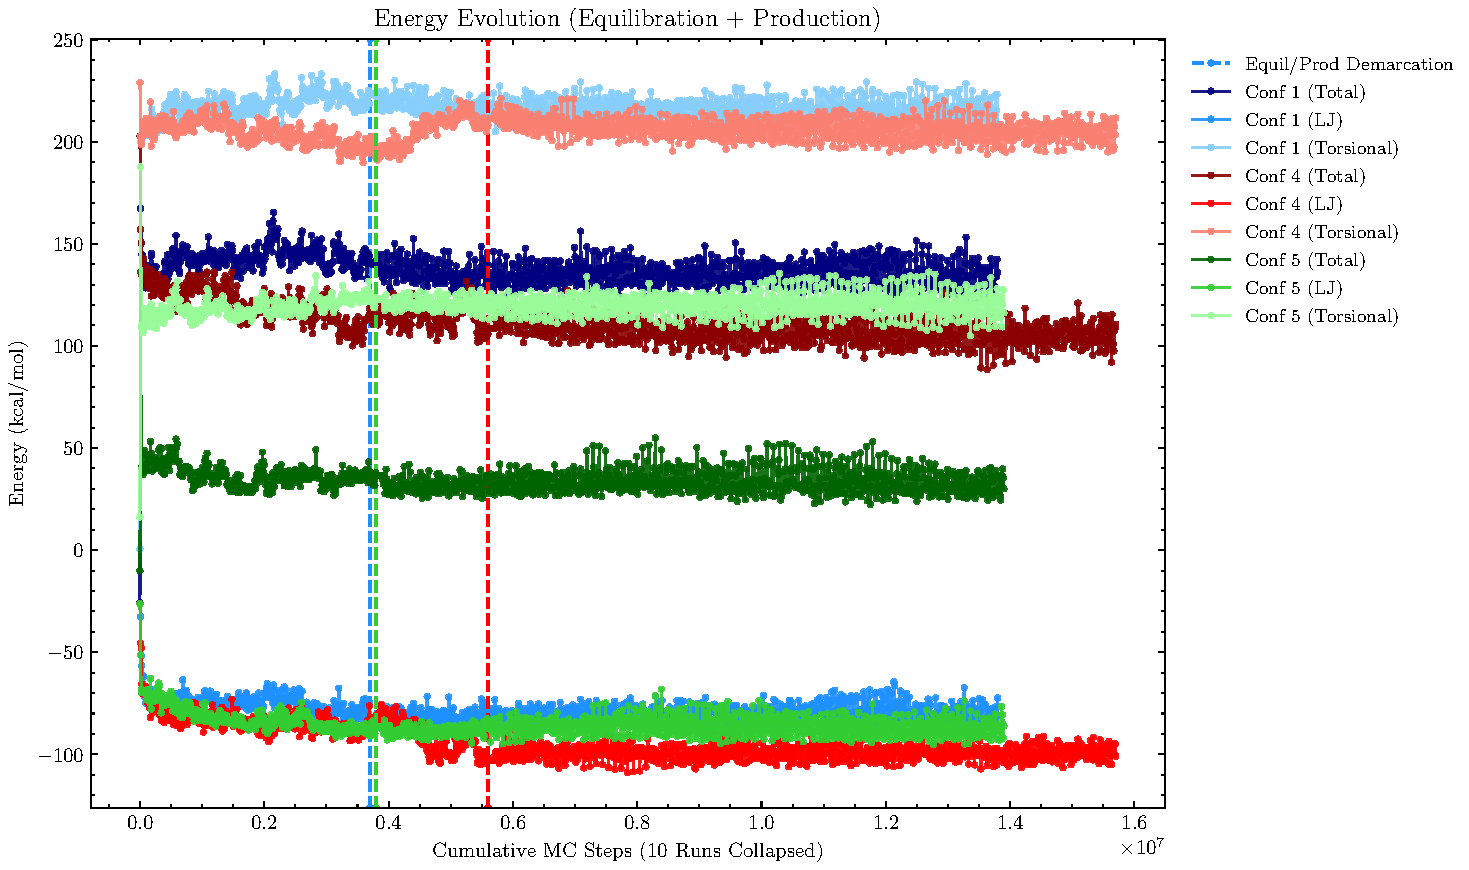
\includegraphics[width=0.8\textwidth]{figs/parallel_combined/parallel_energy_evolution.pdf}
  \caption{Total, LJ, \& Torsional Energy plots across various initial
    conformations}
  \label{fig:par_energy}
\end{figure}

Figure \ref{fig:par_energy} tracks the total, Lennard-Jones (LJ), and torsional energy
trends over the progression of Monte Carlo Steps (MCS) for
configurations 1, 4, and 5. The vertical dashed lines mark the
transition point between equilibration and the subsequent 10-million
step production data. 

In this particular instance of the combined
simulation, the torsional and LJ energy took longer to stabilize in
configuration 4 than the other configurations (1 \& 5), meaning
equilibration took longer to pass the Geweke equilibration determination
test as indicated in the red, vertical, dashed line. For this reason
its combined simultion to run for ${\sim}1.55 \times 10^7$ total steps.

An important observation and detail obtained from this graph is how
initial configuration influences the total energy within the simulation.
Configurations 1 \& 4 are rigid and straight helical structures,
respectively, while introducing random, out-of-plane tilts to
configuration 5 allowed it to find a much lower equilibrated torsional
(and therefore, total) energy.

\begin{figure}[H]
  \centering
  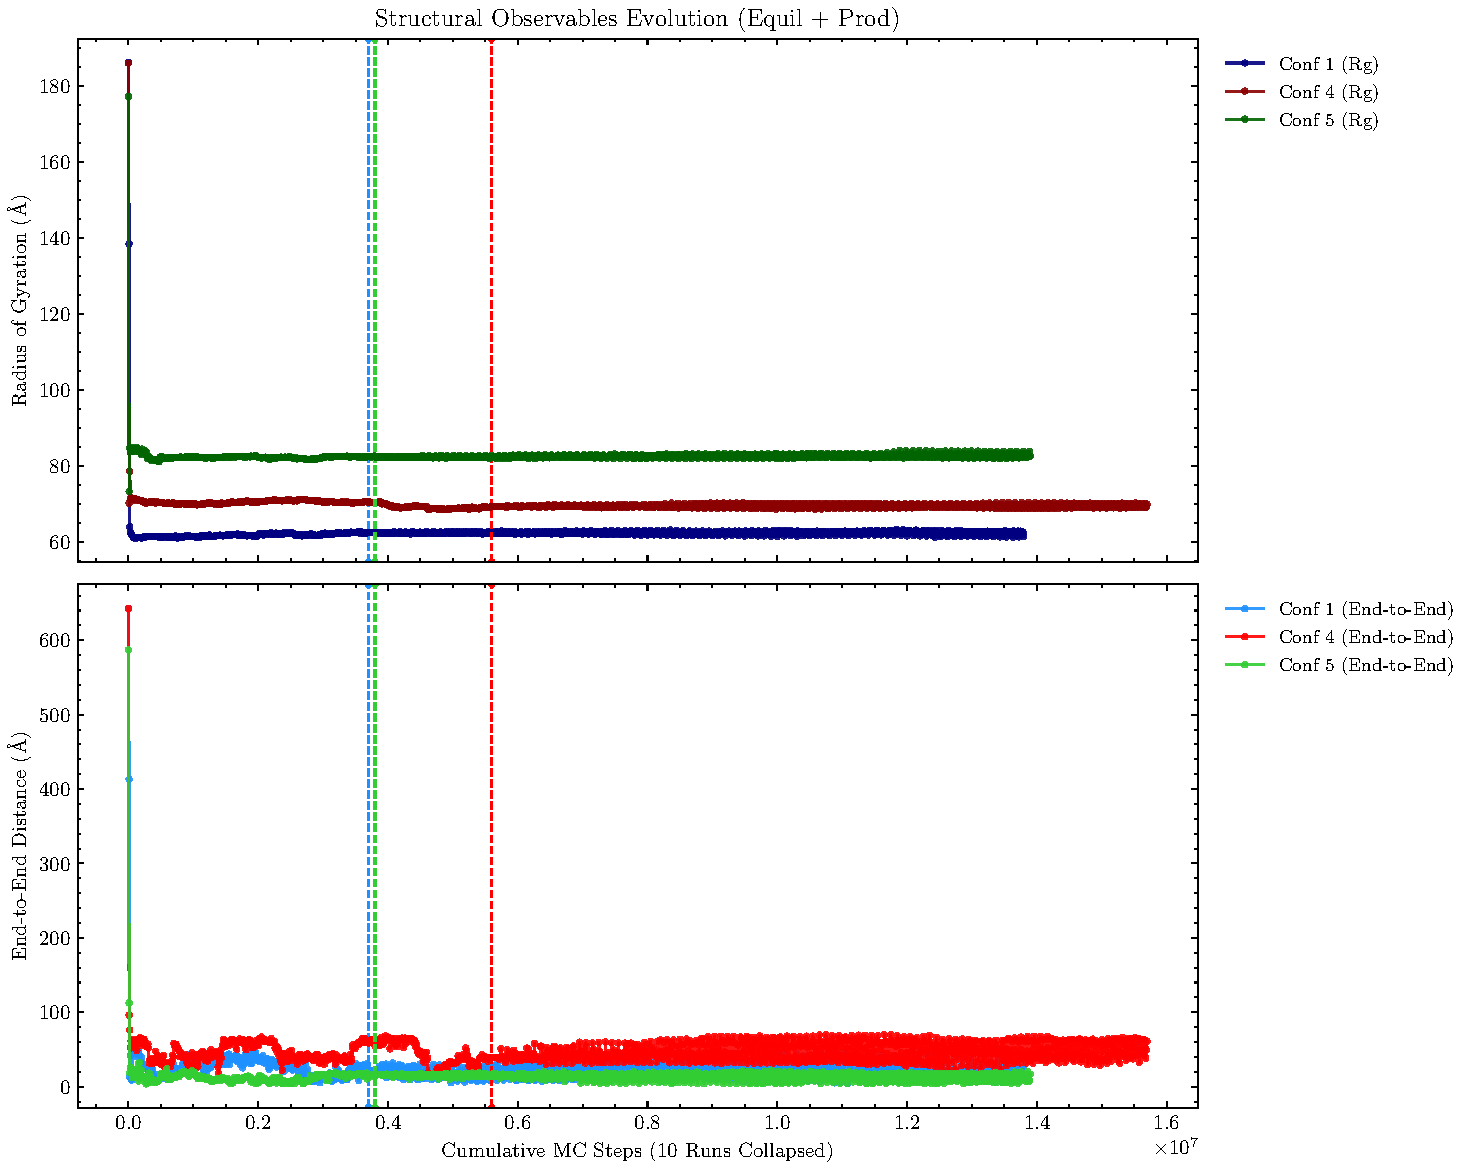
\includegraphics[width=0.8\textwidth]{figs/parallel_combined/parallel_observables_evolution.pdf}
  \caption{Radius of Gyration \& End-to-End Distance plots across
    various initial conformations}
  \label{fig:par_obs}
\end{figure}

Figure \ref{fig:par_obs} displays the Radius of Gyration (Rg) and End-to-End Distance
for the different configurations. As with the energy plots above which
showed similar torsional energies between Conf 1 \& 4 while Conf 5 was
much lower after equilibration, the Rg for Conf 5 is the most distinct
here as well. Configuration 5, due to its initial out-of-plane tilts,
was able to better relax its bonds into low-energy rotational valleys,
allowing the chain to naturally untangle and adopt an expanded, looser
geometry, mathematically resulting in a higher Radius of Gyration.

\begin{figure}[H]
  \centering
  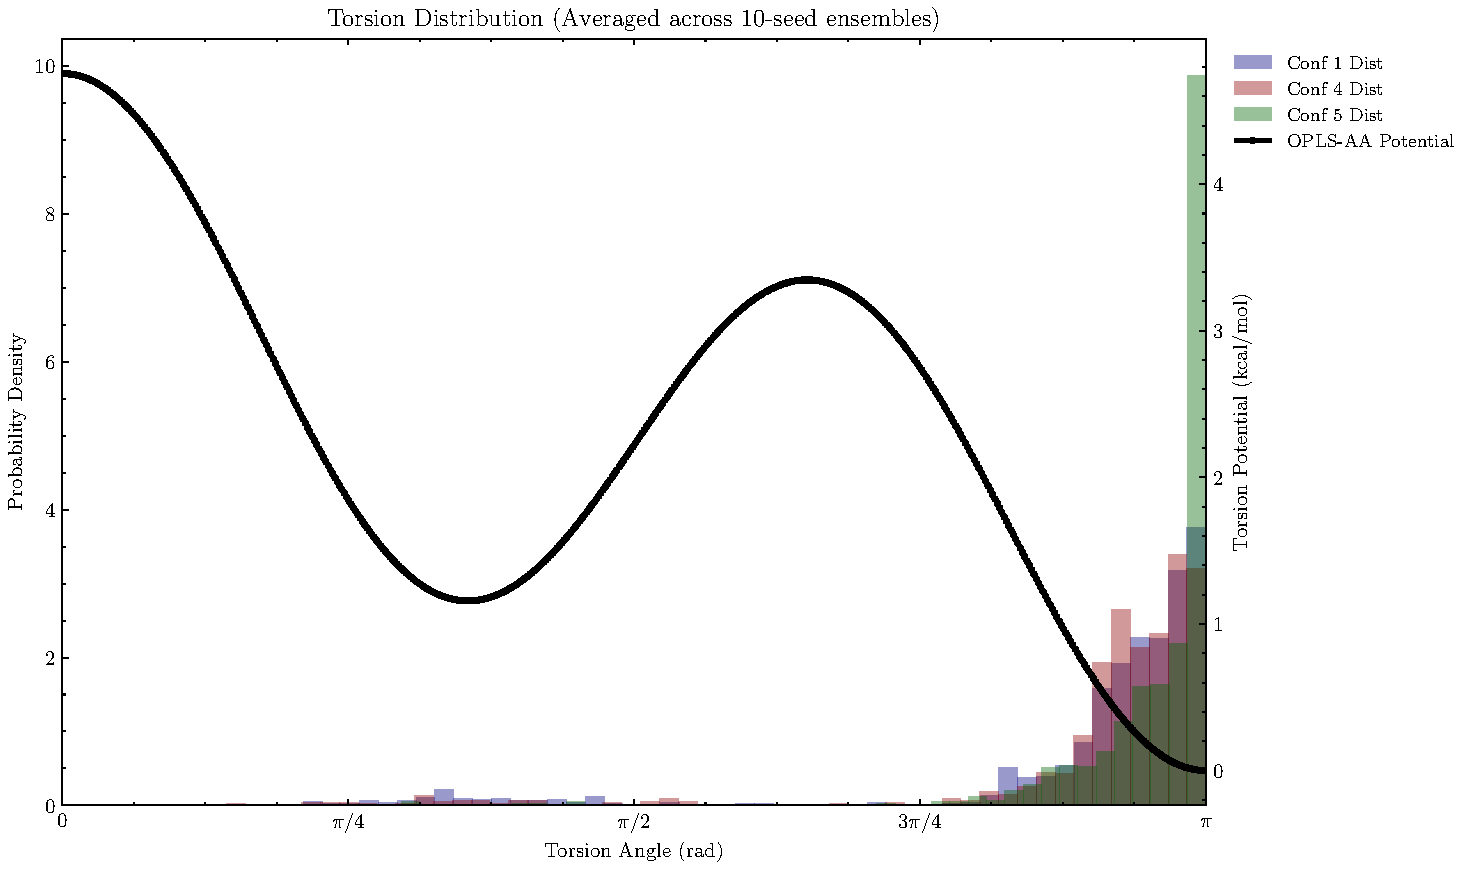
\includegraphics[width=0.8\textwidth]{figs/parallel_combined/parallel_torsion_distribution.pdf}
  \caption{Torsional distribution of post-equilibrated MCS across
    various initial conformations}
  \label{fig:par_torsion}
\end{figure}

The low-energy rotational valley relaxation tendency for Conf 5 is even
more apparent in figure \ref{fig:par_torsion}, which shows the probability density of the
each polymer exploring various dihedral (torsion) angles. Each
configuration's post-equilibration data is compared to the OPLS-AA
potential, where the results confirm the highest probability at $\pi$
(trans) configuration. While all configurations follow the expected
potential, Conf 5 adheres most closely, fully affirming the above energy
and observable data. Also of note is how the graph demonstrates the
expected rise in probablity around the potential's local minima at
${\sim}\pi/3$.
% Source ownership:
% - Arthur: conclusions


\section{Conclusions}
\label{sec:conclusions}

\subsection{Computer Simulation vs.\ Real-World Results}

While this Monte Carlo simulation successfully modelled the
conformational sampling of a polymer chain, it is important to
recognise the limitations when comparing theoretical calculations
to real-world experimental results.

\begin{itemize}
  \item By employing the OPLS-AA and TraPPE-UA force fields, we gain
    robust mathematical approximations of energy landscapes; however,
    these empirical potentials cannot fully capture the dynamic
    complexities of real-world solvent interactions or subtle quantum
    effects.
  \item The isolation of a single polymer chain within the simulation
    neglects the significant impact of intermolecular forces and
    environmental factors that would be present in a real-world
    scenario.
  \item The all-atom energy module applies a uniform backbone-position threshold
    to suppress short-range non-bonded interactions, which over-excludes some 1-5 and 1-6 hydrogen--hydrogen contacts. The impact is partially mitigated by the torsional potential and the single-chain, vacuum context of the simulation. Nonetheless, this represents a known approximation whose correction is left for future work.
\end{itemize}

\subsection{Nonlinearity of Parallel Speedup}

One of the key observations from our performance analysis is that
parallelisation rarely translates evenly into a 1:1 linear speedup.
In a perfect scenario, assigning four cores would make the code run
four times faster. However, as seen in our MPI benchmarks, adding
more workers inherently introduces communication overhead. The time
required for the orchestrator to pass messages, synchronise
coordinates during ensemble sampling, and track dynamic convergence
tests gradually eats into the raw processing speed. At certain
hardware boundaries, communication bottlenecks and competition for
physical system resources make additional core count benefits
negligible.

\subsection{Navigating Resource Utilization}

Combining multiple High-Performance Computing (HPC) methodologies --
such as MPI and OpenMP -- offers significant acceleration capabilities,
but requires careful resource management to prevent oversubscription.
Breaking up the simulation workflow into phases proved to be a critical
step in reusing resources and limiting the system size required to run
the program.

\subsection{HPC Optimization}

Ultimately, achieving high performance is not simply a matter of
checking whether a particular parallel processing technique outpaces
its serial counterpart; rather, it requires a coordinated benchmarking
strategy. Optimizing an HPC code ecosystem demands careful evaluation
of how different techniques overlap and complement one another. Were
this a commercial or funded research project, benchmarking the
performance of the various technique combinations (and against the
system hardware available) would be prudent.

Figure \ref{fig:scheme} illustrates our parallel processing architecture,
which leverages a central Master Node to efficiently orchestrate tasks
across the system. With combined optimization and parallelization
techniques, a possible workflow functions as follows:

\begin{itemize}
  \item The Master Node checks if an equilibrated geometry already
    exists, allowing it to bypass the computationally heavy equilibration
    phase for previously processed configurations (such as Conf 4, which
    immediately unlocks its production runs).
  \item For new configurations (like Confs 1 and 5), the system
    simultaneously deploys independent replicas.
  \item These replicas utilize a collaborative swarm logic, aided by
    the Geweke Convergence test running on 2 workers with 2 threads
    each, to dynamically find equilibrium as fast as possible.
  \item Since an equilibrated geometry for conformation type 4 is
    already supplied, the 2 workers with their 2 OpenMP threads each
    are immediately available to assist in the production runs for
    that configuration.
  \item Meanwhile equilibration completes for conformations 4 \& 5,
    and those workers become available to start assisting in the
    remaining jobs from the shared 30-job global production queue.
\end{itemize}

Total core count for this scenario (default when the parallel
submission script is invoked) is \textbf{13 cores}:

\begin{itemize}
  \item \textbf{1} Master Node (\textbf{1 core})
  \item 2 Workers each running a Conformation Equilibration
    \begin{itemize}
      \item Each of these workers takes 2 cores for Swarm Logic
        \begin{itemize}
          \item Each node calculates energy via 2 OpenMP threads
            ($2\times2\times2=$ \textbf{8 cores})
        \end{itemize}
    \end{itemize}
  \item 2 Workers immediately start production runs on
    equilibration-bypassed conformation~\#4. (\textit{Why 2? The
    system opts to utilize the same number of workers for a bypassed
    configuration as it would a swarm-logic equilibration.})
    \begin{itemize}
      \item These workers' energy calculations are threaded with
        OpenMP ($2\times2=$ \textbf{4 cores})
    \end{itemize}
  \item When the equilibration phase is done for conformations 1 \& 5,
    those workers are reassigned unfinished chunks of the production
    queue, \textit{reusing the CPU resources}, 4 cores per conformation.
    (\textbf{+0 cores})
  \item As workers finish their subtasks, they inform the orchestrator,
    receiving any pending jobs from the global queue until all 30
    production jobs are completed. (\textbf{+0 cores})
\end{itemize}

\begin{figure}[H]
  \centering
  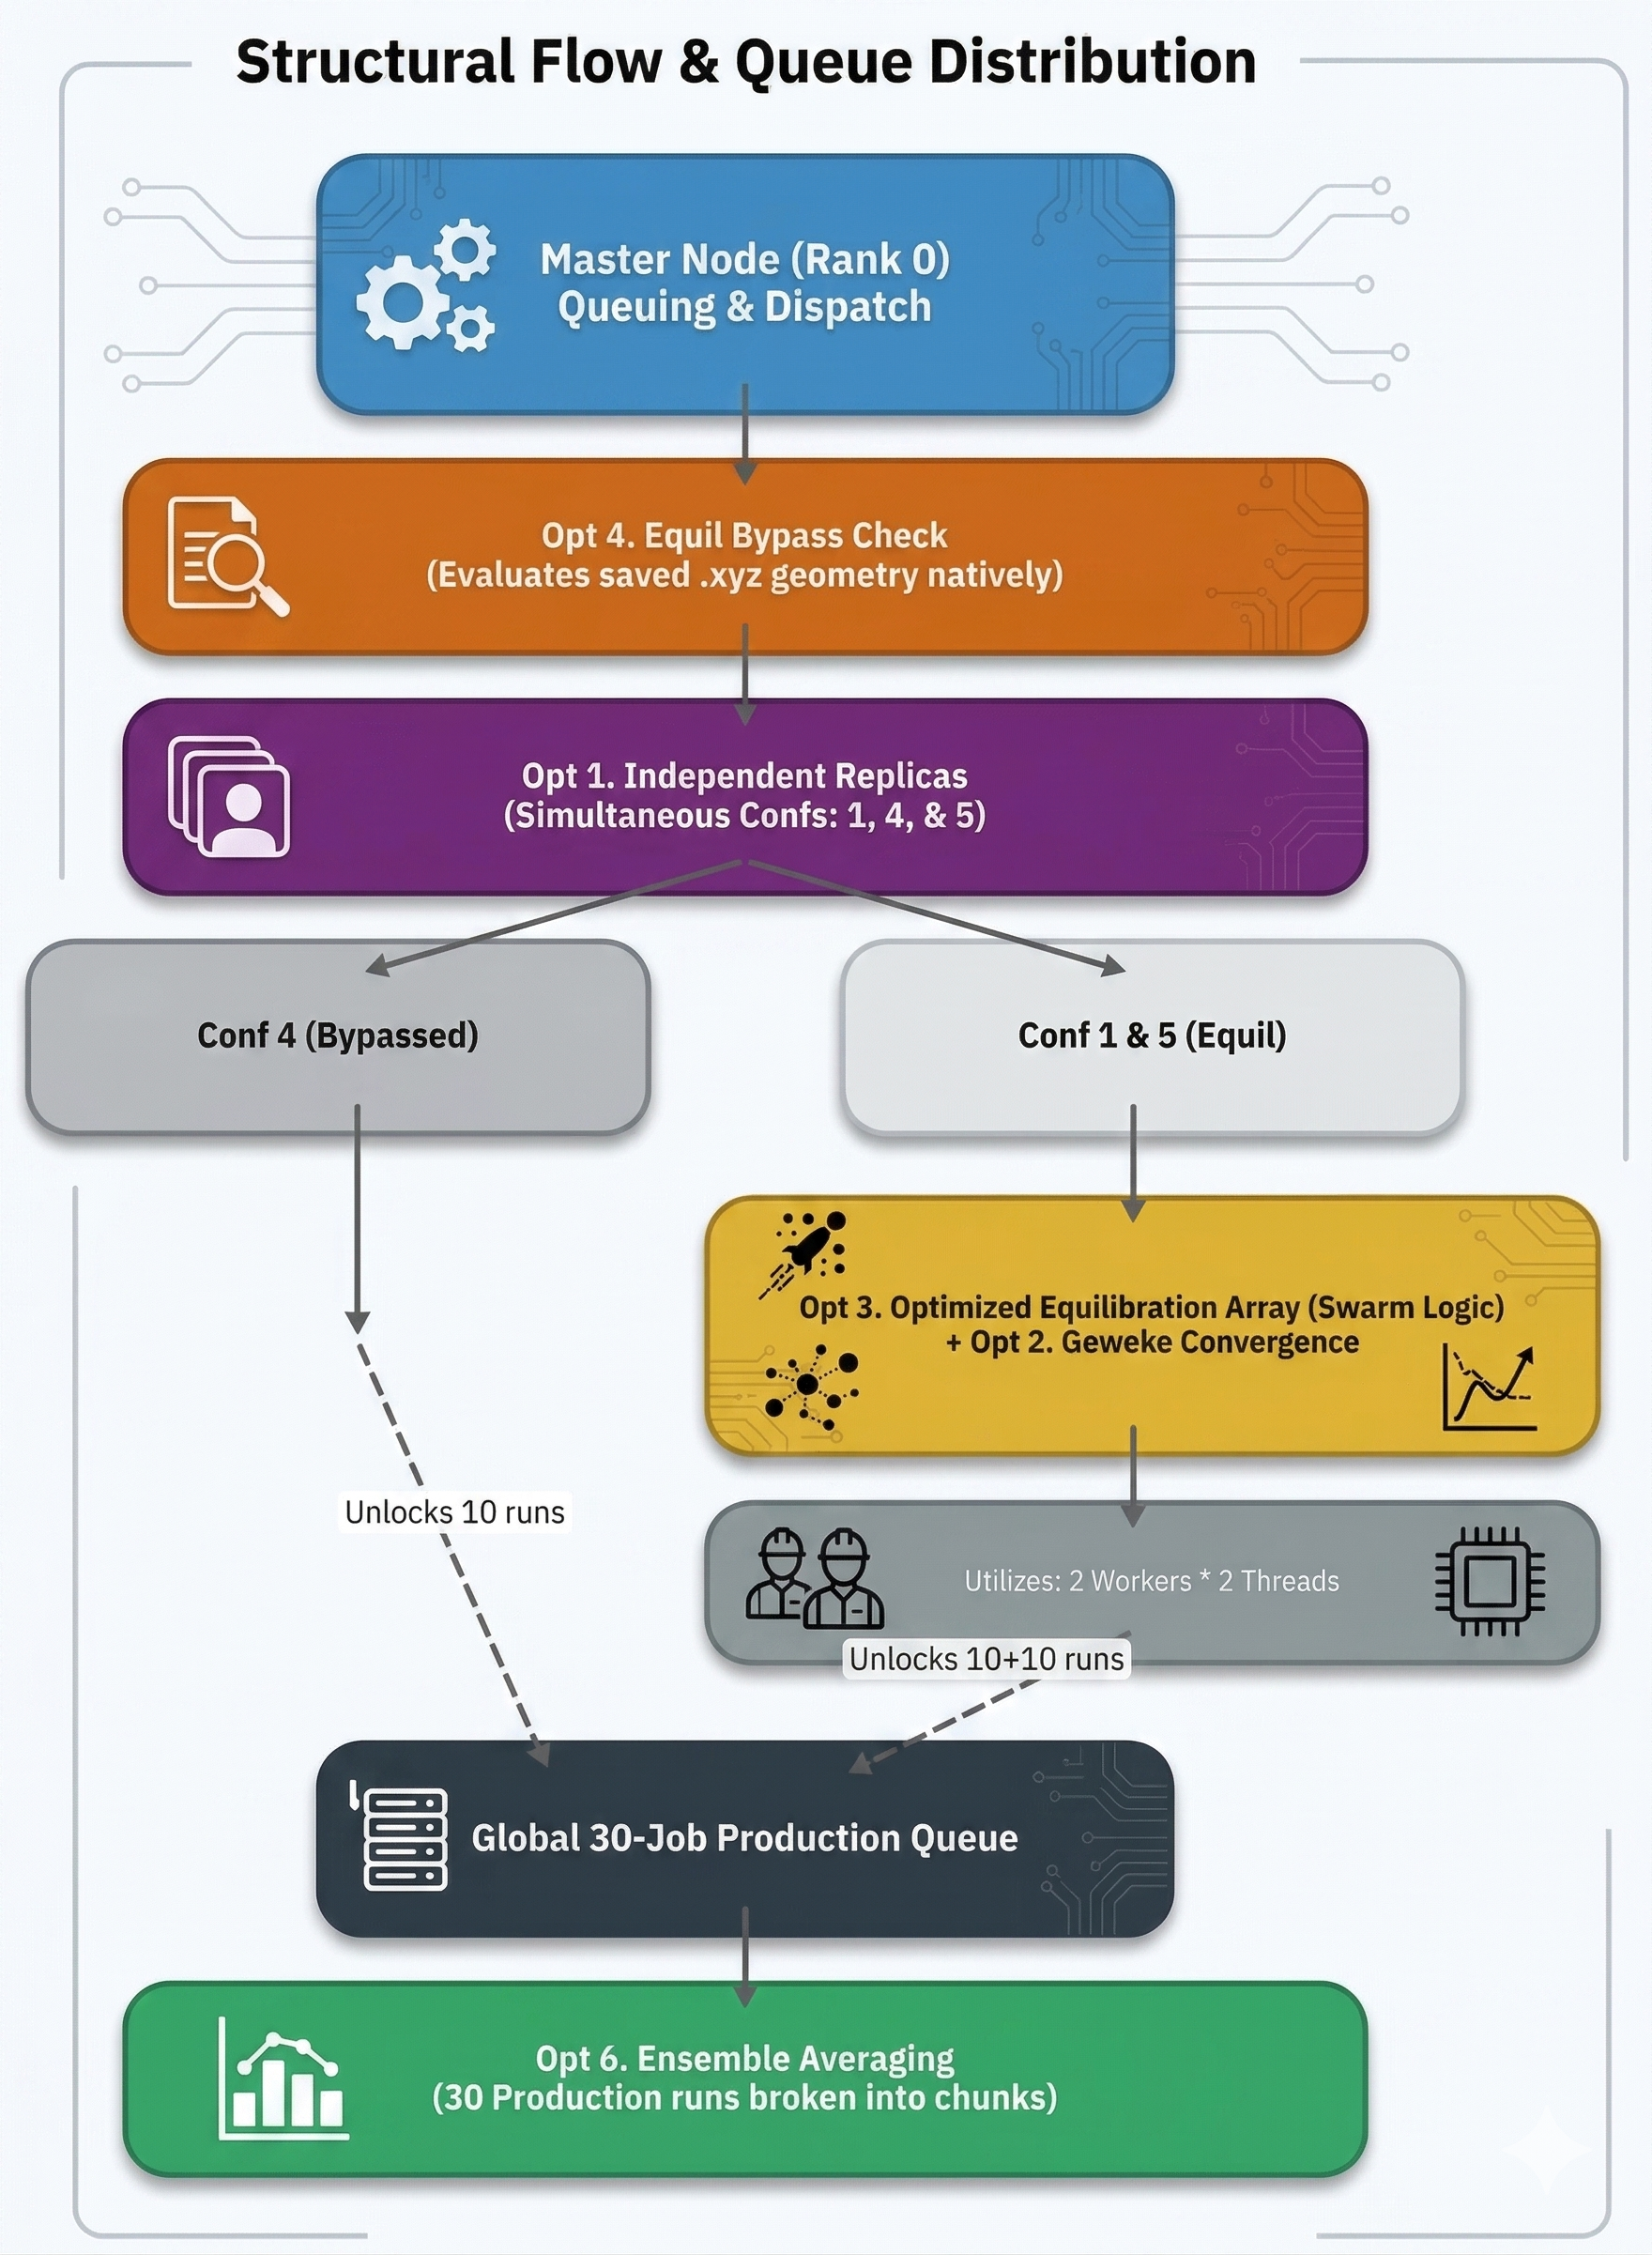
\includegraphics[width=0.8\textwidth]{ParallelProcessing_ResourceUtilization.png}
  \caption{Schematic view of the combined MPI/OpenMP resource utilization strategy.}
  \label{fig:scheme}
\end{figure}

\subsection{Wall Clock Comparison: Parallel vs Serial}

\begin{figure}[H]
  \centering
  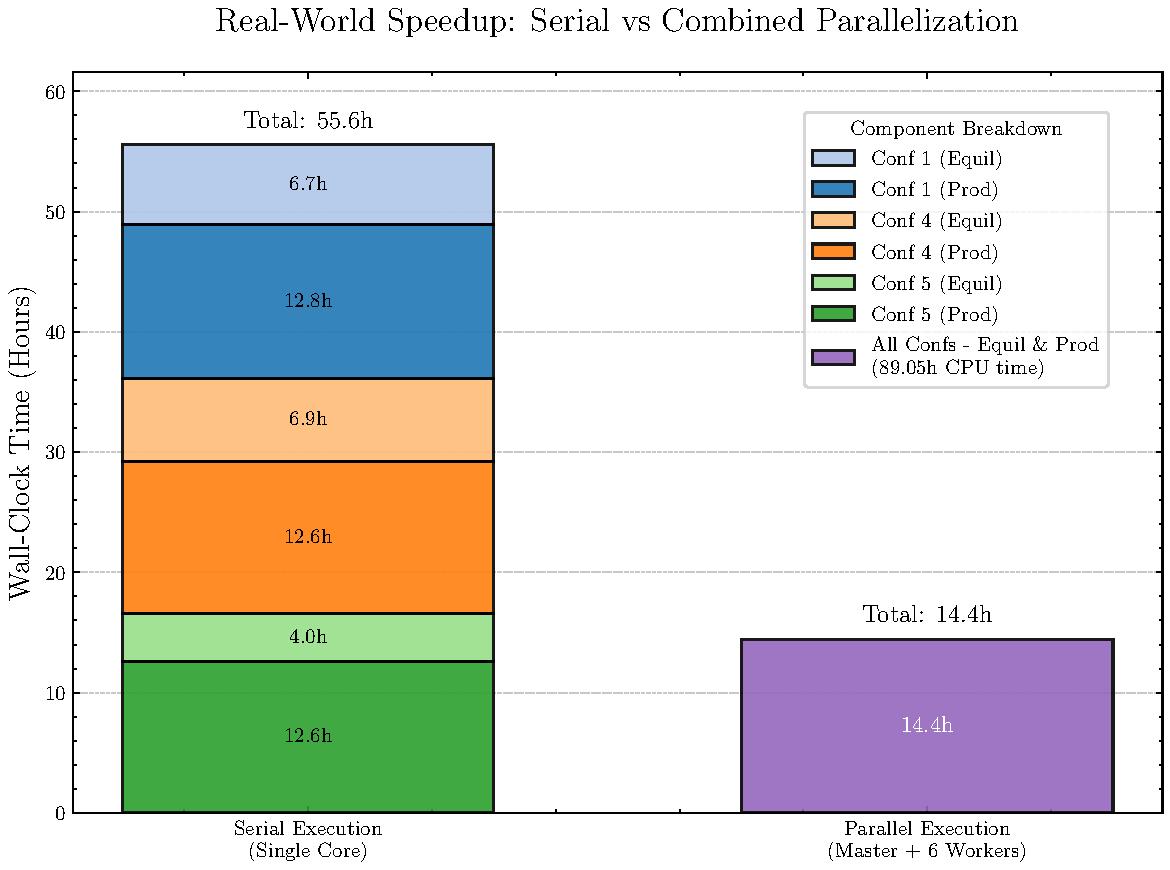
\includegraphics[width=0.8\textwidth]{figs/parallel_combined_v_serial_plot.pdf}
  \caption{Wall-Clock timing for serial vs combined parallelized simulation}
  \label{fig:par_v_ser}
\end{figure}

A final test of the parallelization efforts' efficiency was running the simulation serially, combining their runtimes, and comparing it to the wall-clock time required to complete the same parallel execution. No equilibration steps were bypassed to keep the comparison as similar as possible.

As seen in figure \ref{fig:par_v_ser}, the parallel version took 14h 26min to complete while the serial versions took a combined 55h 35m to perform the same tasks. The parallel version required 13 cores to operate, consisting of over 89h of compute time, not counting the master node's orchestration. The multi-processing approach condensed the parallel version's CPU-to-Wall clock time by a factor of \textbf{6.16x}, while the wall-to-wall clock speedup (parallel vs serial) was sped up by \textbf{3.85x}.

It's interesting to notice that while more resources are needed to run the parallel version, it was also able to complete all 3 configurations' equilibration and production simulations faster than the quickest serial simulation (Conf 5). This beautifully illustrates the contributions of high-performance computing architecture to scientific research, showing that it can assist in converting multi-day research bottlenecks into overnight jobs.
\input{sections/15_references}

\end{document}